\documentclass[prodmode,acmtcps]{acmsmall}

% Metadata Information
\acmVolume{9}
\acmNumber{4}
\acmArticle{39}
\acmYear{2016}
\acmMonth{7}

\usepackage{graphicx}
%\graphicspath{{figs/}}
\usepackage{paralist}
\usepackage{todonotes}  %\newcommand{\todo}[][a]{}
\usepackage{color}
\usepackage{epstopdf}
\usepackage{subfigure}
\usepackage{amssymb}
\usepackage{amsfonts}
\usepackage{cool}  % COntext-Oriented math for LaTeX
\usepackage{mleftright}  % Commands \mleft and \mright
\usepackage{booktabs}
%\usepackage{subfloat}
\usepackage[per-mode=symbol]{siunitx}
\usepackage{url}


\usepackage{hyperref}
\hypersetup{citecolor=black, colorlinks=false}
\usepackage[font=small]{caption}
\usepackage{cite}

% Also, note that the amsmath package sets \interdisplaylinepenalty to 10000
% thus preventing page breaks from occurring within multiline equations. Use:
%\interdisplaylinepenalty=2500
% after loading amsmath to restore such page breaks
\usepackage{comment}
\usepackage[amsmath,thmmarks,thref]{ntheorem}
\usepackage{algorithm,algpseudocode}
\theoremstyle{definition}
\newtheorem{observation}{Observation}
\usepackage{truonglatexdefs}

\usepackage{enumitem, kantlipsum}
\usepackage{tikz}
\usetikzlibrary{arrows}
\tikzset{
  treenode/.style = {align=center, inner sep=0pt, text centered},
  branch_c/.style = {treenode, circle, black, draw=black,
    text width=1.5em, very thick},  
  branch_l/.style = {treenode, circle, blue!50!gray!, draw=blue!50!gray!,
    text width=1.5em, very thick},
  branch_r/.style = {treenode, circle, red!50!gray!, draw=red!50!gray!, 
    text width=1.5em, very thick},
}

%\usepackage{balance}
\def\u{\mathrm{u}}
\def\x{\mathrm{x}}
\def\y{\mathrm{y}}

%\usepackage{etoolbox}
%\makeatletter
%\patchcmd{\maketitle}{\@copyrightspace}{}{}{}
%\makeatother

%\apptocmd{\thebibliography}{\small}{}{}

\begin{document}
% Page heads
\markboth{A. Jain et al.}{Data-driven Model Predictive Control with Regression Trees -- \\
	An Application to Building Energy Management}

% Title portion
\title{Data-driven Model Predictive Control with Regression Trees --\\
	An Application to Building Energy Management}
\author{ACHIN JAIN
\affil{University of Pennsylvania}
FRANCESCO SMARRA
\affil{Universit\`{a} degli Studi dell'Aquila}
MADHUR BEHL
\affil{University of Virginia}
RAHUL MANGHARAM
\affil{University of Pennsylvania}}

% NOTE! Affiliations placed here should be for the institution where the
%       BULK of the research was done. If the author has gone to a new
%       institution, before publication, the (above) affiliation should NOT be changed.
%       The authors 'current' address may be given in the "Author's addresses:" block (below).
%       So for example, Mr. Abdelzaher, the bulk of the research was done at UIUC, and he is
%       currently affiliated with NASA.

\begin{abstract}

\textcolor[rgb]{0.00,0.00,1.00}{Large-scale cyber-physical systems optimization is one of the most important problems nowadays, therefore the use of optimal control strategies is fundamental. Model Predictive Control (MPC) is a control strategy based on the ability to predict system's behavior, that provides optimal solutions in order to optimize a generic system performance while ensuring system's constraints. For this reason MPC represents the best solution to optimize systems' performance. However, the main bottle neck that does not allow the widespread of predictive control algorithms for complex systems is mainly due to their complexity. This is because the resulting cost and time efforts needed to construct system models, as for example in the case of buildings, is prohibitive. To address this issue, a regression trees-based approach is introduced in this paper. More precisely, a data-driven model predictive control based on regression trees is proposed, which allows to perform closed-loop optimal control synthesis for cyber-physical systems. In this paper, such methodology is used to face the Demand-Response problem in buildings. In particular, it is used to optimally trade off peak power reduction against thermal comfort without having to learn white/grey box models of the systems dynamics.}
\end{abstract}


%
% The code below should be generated by the tool at
% http://dl.acm.org/ccs.cfm
% Please copy and paste the code instead of the example below. 
%
\begin{CCSXML}
<ccs2012>
<concept>
<concept_id>10010147.10010257.10010293.10003660</concept_id>
<concept_desc>Computing methodologies~Classification and regression trees</concept_desc>
<concept_significance>500</concept_significance>
</concept>
</ccs2012>
\end{CCSXML}

\ccsdesc[500]{Computing methodologies~Classification and regression trees}


%
% End generated code
%

% We no longer use \terms command
%\terms{Design, Algorithms, Performance}

\keywords{Machine learning; Predictive control; Cyber-physical Systems; Demand response; Peak power reduction}

\acmformat{Achin Jain, Francesco Smarra, Madhur Behl and Rahul Mangharam, 2016. Data-driven Model Predictive Control with Regression Trees -- An Application to Building Energy Management.}

% At a minimum you need to supply the author names, year and a title.
% IMPORTANT:
% Full first names whenever they are known, surname last, followed by a period.
% In the case of two authors, 'and' is placed between them.
% In the case of three or more authors, the serial comma is used, that is, all author names
% except the last one but including the penultimate author's name are followed by a comma,
% and then 'and' is placed before the final author's name.
% If only first and middle initials are known, then each initial
% is followed by a period and they are separated by a space.
% The remaining information (journal title, volume, article number, date, etc.) is 'auto-generated'.

\begin{bottomstuff}
Author's addresses: {A. Jain {and} R. Mangharam, Department of Electrical and Systems Engineering,
University of Pennsylvania; 
F. Smarra, Department of Information Engineering, Computer Science and Mathematics, Universit\`{a} degli Studi dell'Aquila;
M. Behl, Department of Computer Science, University of Virginia.
This work was partially supported by the Italian Government under Cipe resolution n.135 (Dec. 21, 2012), project \emph{INnovating City Planning through Information and Communication Technologies} (INCIPICT).}
\end{bottomstuff}

\maketitle

\section{Introduction}
\label{sec:intro}
2015 was the hottest year on record since the beginning of weather recording in 1880~\cite{noaa}. Heat waves in summer and polar vortexes in winter are growing longer and pose increasing challenges to an already over-stressed electric grid. Furthermore, with the increasing penetration of renewable generation, the electricity grid is also experiencing a shift from predictable and dispatchable electricity generation to variable and non-dispatchable generation. This adds another level of uncertainty and volatility to the electricity grid. The volatility due to the mismatch between electricity generation and supply further leads to volatility in the wholesale price of electricity. For example, the polar vortex triggered extreme weather events in the U.S. in January 2014, which caused many electricity customers to experience increased costs. Parts of the U.S. north-eastern electricity grid experienced a 86-fold increase in the price of electricity from $\$31/\si{\mega\watt\hour}$ to $\$2,680/\si{\mega\watt\hour}$ in a matter of a few minutes~\cite{volatility}.  Such events show how unforeseen and uncontrollable circumstances can greatly affect electricity prices that impact grid operator and customers. Electricity price volatility, is becoming the new norm rather than the exception.

Across the United States, utilities and grid operators are devoting increasing attention and resources to Demand-Response (DR). It is considered as a reliable means of mitigating the uncertainty and volatility of renewable generation and extreme weather conditions and improving the grid's efficiency and reliability. The resource contribution from all U.S. DR programs is estimated to be nearly 72,000 MW, or about 9.2 percent of U.S. peak demand~\cite{federal2008assessment} making DR the largest virtual generator in the U.S. national grid. The annual revenue to end-users from DR markets with PJM ISO alone is more than \$700 million~\cite{pjm}. Global DR revenue is expected to reach nearly \$40 billion from 2014 through 2023~\cite{navigant}.

The volatility in real-time electricity prices poses the biggest operational and financial risk for large scale end-users of electricity such as large commercial buildings, industries and institutions, often referred to as \textit{C/I/I} consumers. In order to shield themselves from the volatility and risk of high prices, such consumers must be more flexible in their electricity demand. Consequently, large \textit{C/I/I} customers are increasingly looking to demand response programs to help manage their electricity costs. DR programs involve a voluntary response of a building to a price signal or a load curtailment request from the utility or the curtailment service provider (CSP). Upon successfully meeting the required curtailment level the end-users are financially rewarded, but may also incur penalties for under-performing and not meeting a required level of load curtailment. In practice, one of the biggest challenges with end-user demand response is the following: \emph{Upon receiving the notification for a DR event, what actions must the end-user take in order to achieve an adequate and a sustained DR curtailment?} 

Unfortunately, most of the Demand Response today is done in an ad-hoc manner. 
The decisions are rule-based or they depend upon a building operator's experience, which has several disadvantages:

\begin{itemize}[leftmargin=1cm]
	\item \emph{Limitations of rule-based.} The building's operating conditions, internal thermal disturbances and environmental conditions must all be taken into account to make appropriate DR control decisions, which is not possible with using rule-based and pre-determined DR strategies since they do not account for the state of the building but are instead based on best practices and rules of thumb. 
	Rule based DR strategies have the advantage of being simple but they do not account for the state of the building and weather conditions during a DR event.
	\item \emph{Control complexity and scalability.} Upon receiving a notification for a DR event, the building's facilities manager must determine an appropriate DR strategy to achieve the required load curtailment. 
	These control strategies can include adjusting zone temperature set-points, supply air temperature and chilled water temperature set-point, dimming or turning off lights, decreasing duct static pressure set-points and restricting the supply fan operation \etc. 
	In a large building, it is difficult to assess the effect of one control action on other sub-systems and on the building's overall power consumption because the building sub-systems are tightly coupled.
\end{itemize}
These drawbacks are addressed by predictive control techniques such as Model Predictive Control (MPC). MPC allows to optimize desired performance while guaranteeing system's constraints. For example, it can be used to provide the optimal actions for an energy curtailment during a DR event while guaranteeing thermal comfort for occupants. So MPC-based solutions fit into the DR problem. However, the quality of the MPC solutions depends on the accuracy of the predictive models describing the system. This limits the widespread of MPC for complex systems such as buildings. Thus, in context of modeling of large buildings, applying MPC poses further challenges:

\begin{itemize}[leftmargin=1cm]
\item \emph{Modeling complexity and heterogeneity.} Unlike the automobile or the aircraft industry, each building is designed and used in a different way and therefore it must be uniquely modeled. Learning predictive models of building's dynamics using first principles based approaches (\eg with EnergyPlus~\cite{Crawley2001319}) is very cost and time prohibitive and requires retrofitting the building with several sensors~\cite{costmpc}. The user expertise, time and costs required to develop a model of a single building are very high.
%\item \emph{Interpretability of modeling and control.} Predictive models for buildings, regardless how sophisticated, lose their effectiveness unless they can be interpreted by human experts and facilities managers in the field. Therefore, the required solution must be transparent, human centric and highly interpretable.
\end{itemize}

\subsection{Main contribution}

\textcolor[rgb]{0.00,0.00,1.00}{In order to address the aforementioned challenges, our goal is to use machine learning algorithms to provide data-driven models for cyber-physical systems to take only the advantages of both approaches, i.e. simplicity of rule-based strategies and the predictive capability of model-based control, but without the expense of first principle or grey-box model development. However, this is not an easy task since, although machine learning algorithms are a popular choice for predicting systems' behavior, they do not provide models that are suitable for control. To the best of the authors' knowledge, \cite{Behl201630} is the first work that addresses the problem of using regression tree-based algorithms to provide models of system dynamics to be used in a optimization control problem setup. More precisely, the authors used regression trees-based algorithms to create a data-driven model-based controller for the Demand-Response problem. The authors showed the benefits of using regression trees-based approaches to estimate the DR baseline power consumption and how to build auto-regressive trees for DR control strategies evaluation. Moreover, they proposed a model based control strategy using regression trees (mbCRT) to enable control with regression trees and use it for real-time DR strategy synthesis. In particular, mbCRT algorithm can be used to setup optimal control problems with one-step lookahead prediction, for example to trade off thermal comfort inside a building against the amount of load curtailment. However, mbCRT does not allow to setup a receding horizon control problem with arbitrarily horizon length. This drawback limits closed-loop control performance since it does not take into account the very accurate long term state prediction that regression trees can provide. In this paper we overcome this issue providing the following contributions 
\\
\begin{itemize}[leftmargin=1cm]
	\item \emph{Multi-variate output regression trees:} we introduce a novel methodology to construct a multi-variate output predictive model using regression trees, where each output corresponds to the prediction on a future step of the horizon. More precisely, we setup a least square problem that minimize the prediction error over the control horizon. This is done by modifying the variable selection and splitting criteria at the nodes of the regression tree standard algorithm CART \cite{BreimanFriedmanStoneEtAl1984}.
	\item \emph{Predictive control:} we extend the mbCRT algorithm proposing a Data-driven Predictive Control strategy using Regression Trees (DPCRT), that implements receding horizon control using data-based models learned from the available historical data.
	\item \emph{Application:} we apply this control strategy to peak power curtailment on a large office building and compare with the previous mbCRT algorithm. Results show a substantial improvement using DPCRT by $8.6\%$ with respect of mbCRT in terms of peak curtailment.\\
\end{itemize}
Summarizing,} the methodology proposed in this paper bypass the cost and time prohibitive process of building high fidelity models that use grey and white box modeling approaches while still being suitable for receding horizon control. These are the first algorithms of its kind that enable closed-loop control synthesis and finite receding horizon control with regression trees. \textcolor[rgb]{0.00,0.00,1.00}{Paper flow is summarized in Fig. \ref{F:scheme}.}

\subsection{Related work}
\label{sec:related}
\textcolor[rgb]{0.00,0.00,1.00}{In the recent years a lot of attention has been focused on data-driven optimal control and different approaches have been considered.} For example in some works, models are trained on optimal solutions obtained from MPC. The resulting models can then be used for explicit MPC, as in~\cite{BemporadMorariDuaEtAl2002}. This approach has been applied to problems of  stabilization \cite{CavagnariMagniScattolini1999} and freeway traffic systems using regression trees \cite{OleariFrejoCamachoEtAl2015}. 
Another class of methods solve the optimization directly on the trained models to do predictive control \textcolor[rgb]{0.00,0.00,1.00}{ \cite{Hou2013,Costanzo2016,FerreiraRuanoSilvaEtAl2012}. However, none of them address the problem of including data-driven state models into the optimal predictive control loop, and hence allow to set up a MPC-like optimal control problem. The first results in this sense have been introduced for the first time in \cite{Behl201630}, where the authors proposed MPC-like control problems considering regression tree-based algorithms for the DR problem. In \cite{KusiakSongZheng2009}, instead, neural networks are used to setup a MPC-like control for the wind turbine problem using evolutionary algorithms. Nevertheless, their approaches considered only one-step lookahead predictive model, and hence did not allow predictive control over an arbitrary horizon.}

\textcolor[rgb]{1.00,0.00,0.00}{More specifically to the Demand-Response problem, there is a vast amount of literature like (\cite{oldewurtel2013towards,xu2004peak}), which addresses the problem of determining DR strategies. The majority of the approaches are using either rule-based techniques for curtailment or white/grey box model-based control. These lasts usually assume that the model of the system is either perfectly known or found in literature, whereas the task is much more complicated and time consuming in case of a real building and sometimes, it can be even more complex and involved than the controller design itself. After several years of work on using first principles based models for demand response, multiple authors~\cite{costmpc,reallife} have concluded that the biggest hurdle to mass adoption of intelligent building control is the cost and effort required to capture accurate dynamical models of the buildings. There are ongoing efforts to make tuning and identifying white box models of buildings more autonomous~\cite{new2012autotune}. OpenADR standard and protocol~\cite{openadr} describes the formats for information exchange to facilitate DR but modeling, prediction and control strategies are out of scope. Several machine learning approaches~\cite{edwards2012predicting,vaghefi2014modeling,yin2012scalable} have been utilized before for forecasting electricity load including some which use regression trees. However, there are two significant shortcomings of the work in this area: 
	\begin{inparaenum}[(a)]
		\item these approaches are coarse grained and  are not aimed at solving demand response problems but are restricted to long term load forecasting with applications in evaluating building retrofits savings and building energy ratings; 
		\item  there is no focus on control synthesis or addressing the suitability of the model to be used in control design. 
	\end{inparaenum}
	There exist several different approaches to balance the power consumption in buildings and avoid peaks, e.g. by load shifting and load shedding \cite{KiliccoteEtAl06aca,LeeEtAl08dom}. However, they operate on coarse grained time scales and do not guarantee any thermal comfort.}

\begin{figure}[t!]
	\begin{center}
		\hspace{0.8cm}
		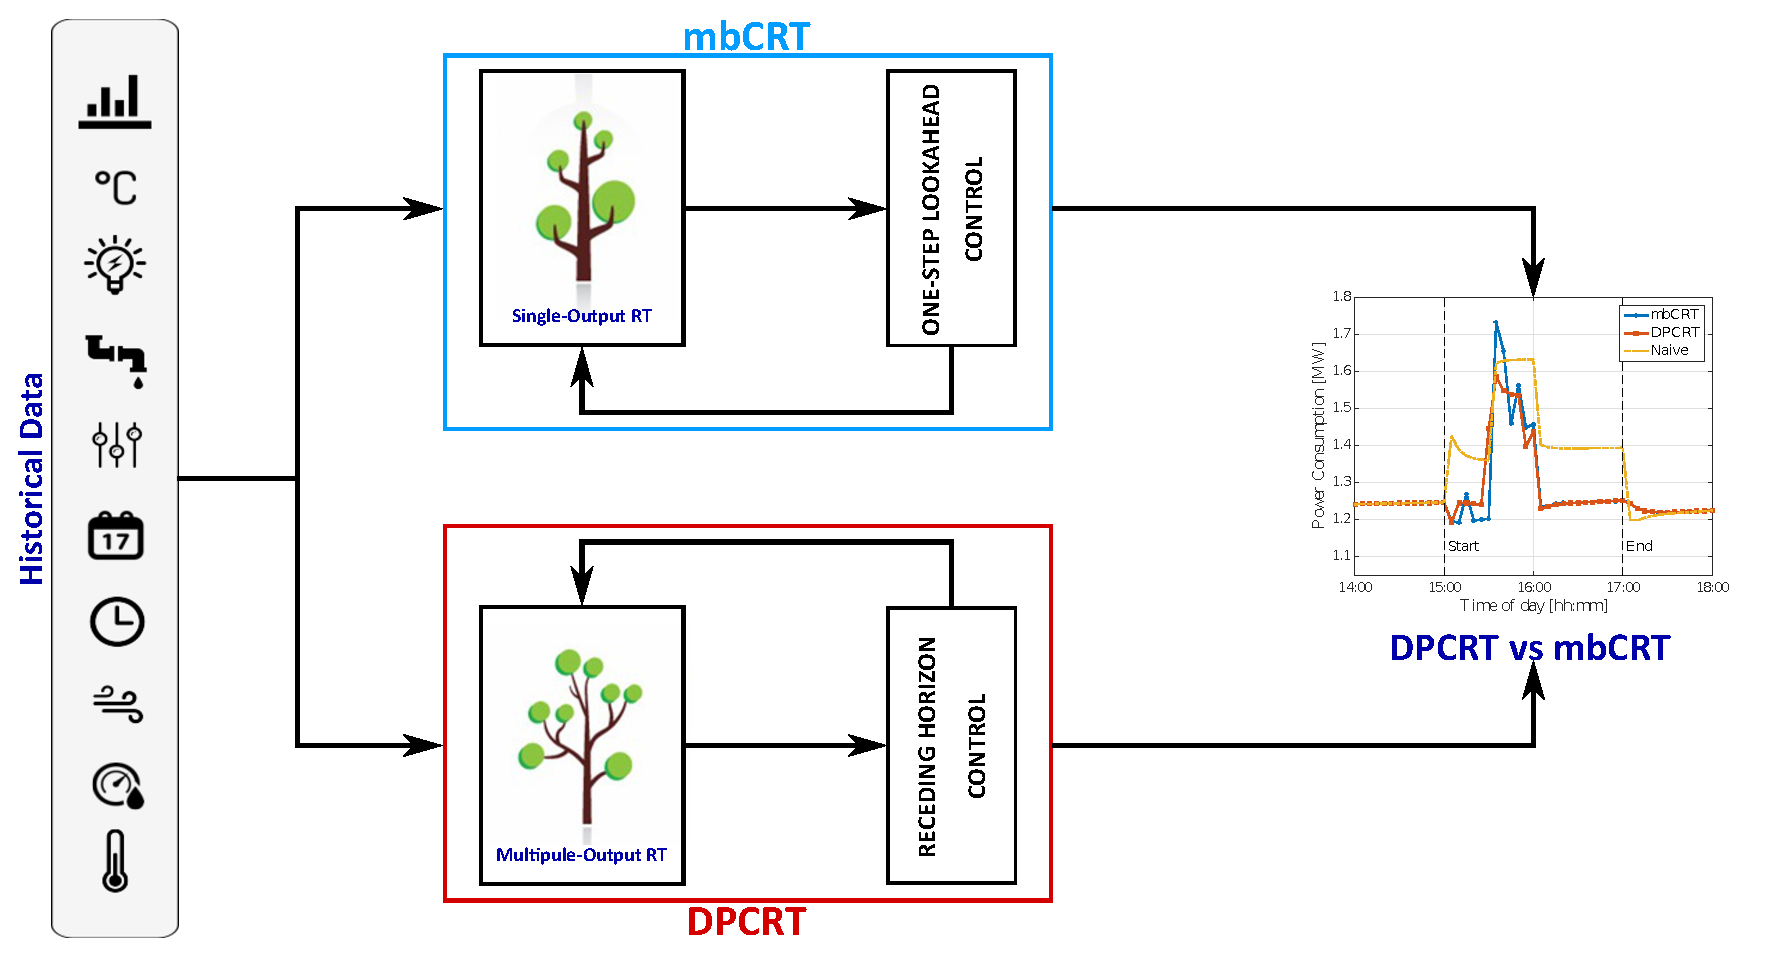
\includegraphics[width=0.8\textwidth]{figs/scheme.eps}
		\centering
		\caption{Historical data are used to train models for both DPCRT and mbCRT. Such models are used to run closed-loop optimization. Finally, the two approaches are compared.}
		\label{F:scheme}
		\vspace{-10pt}
	\end{center}
\end{figure}

The DPCRT algorithm is first of its kind that does finite receding horizon control with regression trees. It is computationally efficient because the optimization problem is convex and the number of constraints scales linearly with the number of control variables. \textcolor[rgb]{0.00,0.00,1.00}{A preliminary version of this paper can be found in the conference paper \cite{JainBuildsys2016}.}

\subsection{Paper organization}

\textcolor[rgb]{0.00,0.00,1.00}{This paper is organized as follows. In Sec.~\ref{sec:problem} we describes our problem formulation. In Sec.~\ref{sec:drtree}, we recall the data-driven control strategy proposed in \cite{Behl201630} that will be useful to introduce our new methodology. In Sec.~\ref{sec:decision_tree} we present our main contribution: predictive control using regression trees. In particular, in Sec. \ref{SS:training_algo} we extend the regression trees standard training algorithm, so that we can use it to build predictive models over an horizon of arbitrary length, while in Sec. \ref{SS:control_tree} we use this algorithm to formally build system models and setup a receding horizon optimal control problem that can be used for the closed-loop control. Finally, in Sec. \ref{sec:case} we apply DPCRT to a peak power reduction problem and compare it with mbCRT.}



\section{Problem Definition}
\label{sec:problem}
\textcolor[rgb]{0.00,0.00,1.00}{Our goal is to find data-driven functional models for cyber-physical systems starting from available historical data. The aim is to build models that relate the value of the response variables $\mathrm{y}_1,\ldots,\mathrm{y}_p$ with the values of the predictor variables or features $\mathrm{x}_1,\ldots,\mathrm{x}_s$, and that can be used to setup an optimization predictive control problem. For example, in the case of buildings the response variables can be represented by the power consumption or the room temperatures, while the features can be represented by weather data, set-points information and building schedules.}
\textcolor[rgb]{1.00,0.00,0.00}{When the dataset has lots of features, as in the case of large buildings, which interact in complicated nonlinear ways, assembling a single global model, such as linear or polynomial regression, can be difficult and lead to poor response predictions. An approach to non-linear regression is to partition the data space into smaller regions $R_i$, where the interactions are more manageable. Regression trees are an example of an algorithm which belongs to the class of recursive partitioning algorithms. The seminal algorithm for learning regression trees is CART as described in~\cite{BreimanFriedmanStoneEtAl1984}. Regression trees-based approaches are our choice to construct data-driven models for cyber-physical systems. The primary reason for this modeling choice is that regression trees are highly interpretable by design. Interpretability is a fundamental desirable quality in any predictive model. Complex predictive models like neural networks, support vector regression \etc go through a long calculation routine and involve too many factors. It is not easy for a human engineer to judge if the operation/decision is correct or not or how it was generated in the first place. For example, building operators are used to operating a system with fixed logic and rules. They tend to prefer models that are more transparent, where it is clear exactly which factors were used to make a particular prediction. At each node of a regression tree, a simple "if this then that" human readable plain text rule is applied to generate a prediction at the leafs, which anyone can easily understand and interpret. Making machine learning algorithms more interpretable is an active area of research, one that is essential for incorporating human centric models in cyber-physical systems.}

\textcolor[rgb]{0.00,0.00,1.00}{We want to use such regression trees-based models to setup optimal predictive control strategies as in the classical MPC formulation. The main problem rising up when dealing with machine learning algorithms is that they do not provide mathematical models that are directly usable for control. To overcome this issue we propose a solution that is based on the \emph{separation of variables}. In particular, given a dataset $(\mathcal{X},\mathcal{Y})$, where $\mathcal{X}=\{\x_1,\ldots,\x_s\}$ is the set of predictor variables (or features) and $\mathcal{Y}=\{\y_1,\ldots,\y_p\}$ is of response variables, we want to use regression trees to learn a model $f_i$ to predict the response $\y_i$ as }
\textcolor[rgb]{0.00,0.00,1.00}{
\begin{equation}\label{eq:RTmodel}
	\y_i=f_i(\x_1,\ldots,\x_s)
\end{equation}
}

\textcolor[rgb]{0.00,0.00,1.00}{
Given a forecast of predictor variables $\hat{\x}_i$, we can predict system response using \eqref{eq:RTmodel}. However, suppose the set of system inputs $\mathcal{X}_c$, that are the variables we can manipulate is a subset of the features set, i.e. $\mathcal{X}_c=\{\mathrm{u}_1,\ldots,\mathrm{u}_m\}\subset\mathcal{X}$. Suppose we want to setup a receding horizon control problem to find optimal inputs that optimize a performance cost function. Let $u(t)=[\mathrm{u}_1(t),\ldots,\mathrm{u}_m(t)]$ be the vector of inputs applied to the system at time $t$ to be optimized, $x(t) = [\mathrm{x}_1(t),\ldots,\mathrm{x}_{s-m}(t)]$ be the vector of system variables measured at time $t$, and $y(t) = [\mathrm{y}_1(t),\ldots,\mathrm{y}_{p}(t)]$ be the vector of system response variables at time $t$, then model \eqref{eq:RTmodel} can not be used to solve the following optimal predictive control problem}

\textcolor[rgb]{0.00,0.00,1.00}{
\begin{equation}\label{eq:linear_program}
\begin{aligned}
& \underset{u_{t+k}\in\mathcal{X}_c}{\text{minimize}} & &  \sum_{k = 0}^{N}{J(y_{t+k},u_{t+k})}  \\
& \text{subject to }                                  & &  y_{t+k}    =   f(x_{t+k},u_{t+k})     \\
&                                                     & &  u_{t+k}   \in \mathcal{\bar U}        \\
&                                                     & &  y_{t+k}   \in \mathcal{\bar Y}        \\
&                                                     & &  x_{t}      =   x(t)                   \\
&                                                     & &  k          =   0,\ldots,N             \\
\end{aligned}
\end{equation}
This is because inputs $u$ are optimization variables, hence they are not known a priori to be used as features to build the prediction using \eqref{eq:RTmodel}.}

\textcolor[rgb]{0.00,0.00,1.00}{
\emph{Separation of variables} is a technique that consists on partitioning the features dataset into inputs (or control variables) and disturbances sets, i.e. the sets of variables we can and can not manipulate, respectively. More precisely, $\mathcal{X} = \mathcal{X}_c\biguplus\mathcal{X}_d$, where $\biguplus$ represents the disjoint union. The regression tree is trained only using the disturbance variables in $\mathcal{X}_d$, so that we can associate to each leaf a model that depends only on the inputs data. In this way we can use disturbances forecasts to predict the system behavior using \eqref{eq:RTmodel}. This procedure provides a modeling framework that allows to solve optimization problem \eqref{eq:linear_program}. In the next $2$ sections we show how this is achieved. In particular, in the next section we recall the mbCRT algorithm, that uses separation of variables to create a regression trees-based model that can be used to solve optimization problem \eqref{eq:linear_program} for the one step lookahead case, i.e. only with $N=0$. Then we provide a novel methodology, based on the redefinition of the regression trees learning algorithm, so that optimization problem \eqref{eq:RTmodel} can be solved for arbitrary $N$. We finally compare in Sec. \ref{sec:case} the performance of the $2$ approaches to show how the long term prediction can improve system performance.}


\section{Control with Regression Trees: Background}
\label{sec:drtree}

In this section we briefly recall the model-based control with regression trees algorithm (mbCRT) proposed in \cite{Behl201630} to synthesize optimal control strategies. 
We provide a general formulation that is suitable for any cyber-physical system.
This will be useful in the next section to introduce our new algorithm. 

\subsection{Data-driven one-step look ahead predictive model}
\label{sec:mbcrt}

\begin{figure}
\centering
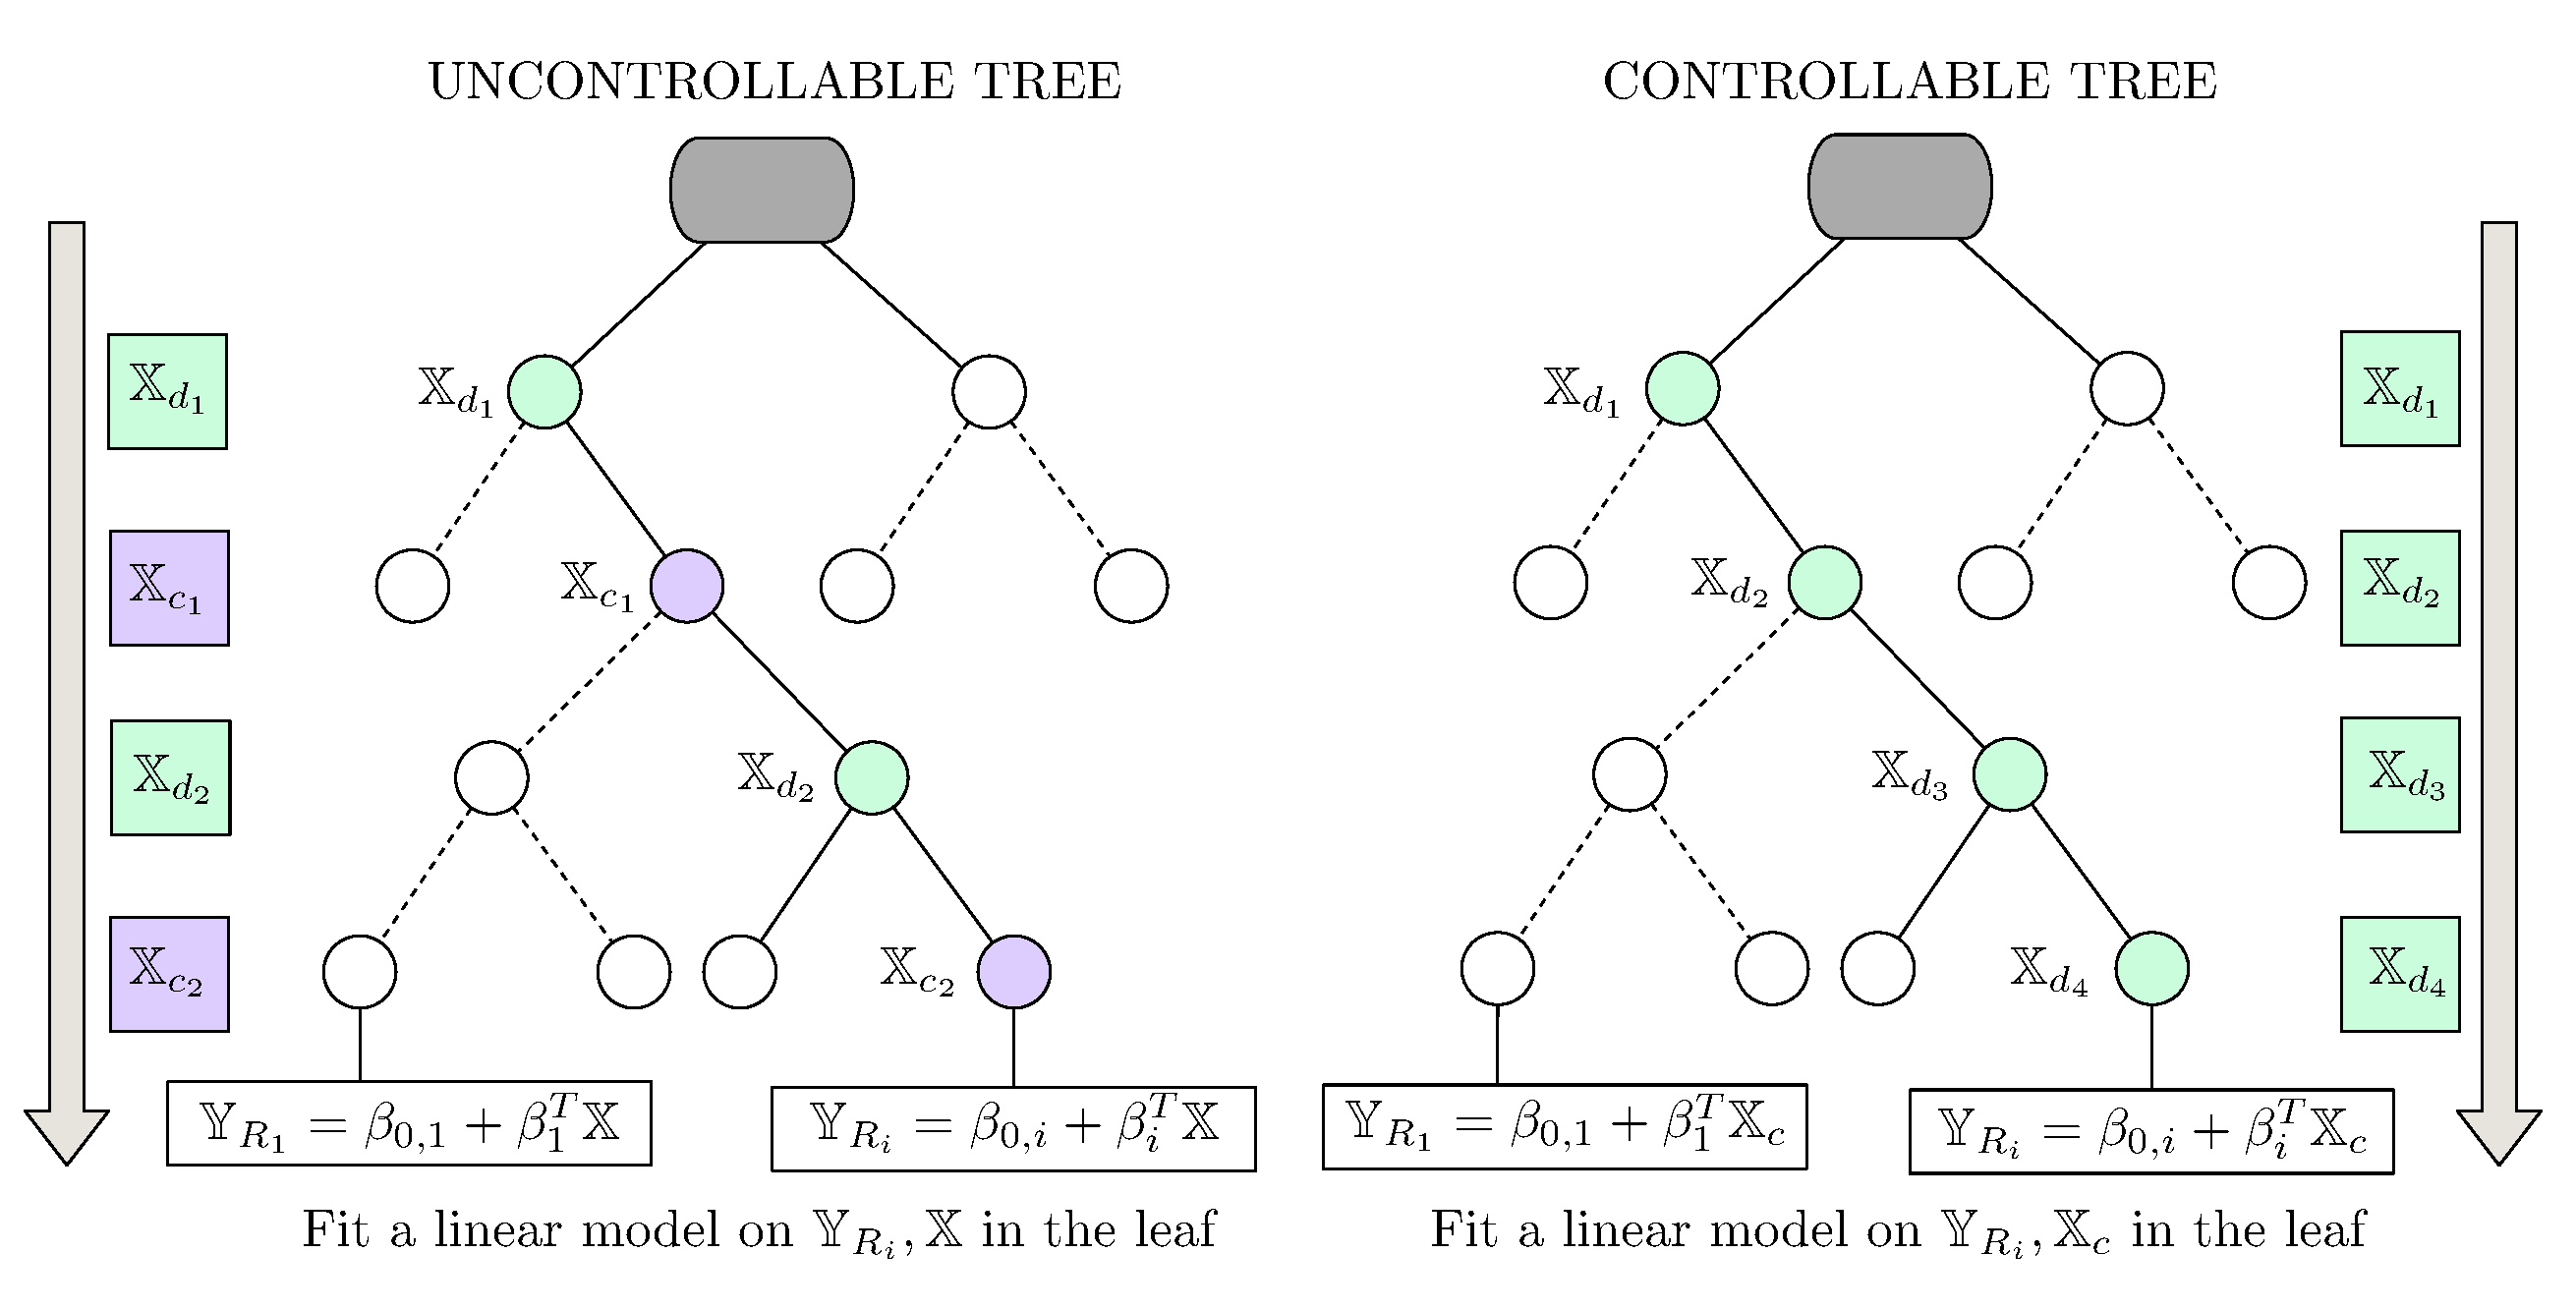
\includegraphics[width=0.9\columnwidth]{Figures/sep_vars.eps}
   \caption{Example of a regression tree not suitable for control due to the mixed order of $\mathcal{X}_c$ and $\mathcal{X}_d$ (left). Example of a tree structure obtained for the mbCRT algorithm. The separation of variables allows using the linear model in the leaf to depend only on the control variables (right).}
   \captionsetup{justification=centering}
   \label{fig:training}
\end{figure}

The \emph{model based Control with Regression Trees (mbCRT)} uses the separation of variables introduced in Sec. \ref{sec:problem}.
The model construction is illustrated in Fig.~\ref{fig:training} -- a regression tree is trained only on disturbance features in $\mathcal{X}_d= \{ \mathrm{d_1,\ldots,d_{s-m}} \} $ to predict the output variable $\mathrm{y}$. Without any loss of generality, we consider only single response variable. 
Multiple trees can be considered for multiple response variables as we do for the case study in Sec.~\ref{sec:case}. 
After learning a regression tree, a linear regression model

\begin{equation}\label{eq:linear_regression_leaf}
\mathrm{y}_{R_\mu} = \beta_{0,\mu} + \beta_\mu u
\end{equation}
is fitted using the subset of samples present in every leaf of the tree, where $\mathrm{y}_{R_\mu}$ is the predicted response in region $R_\mu$ of the tree using all the features in $\mathcal{X}_d$, and $\beta_{0,\mu}\in\mathbb{R}$ and $\beta_\mu\in\mathbb{R}^{1\times m}$. 
Separation of variables allows to use the forecast of the disturbances in $\mathcal{X}_d$ to navigate to the appropriate region $R_\mu$ and use the linear regression model \eqref{eq:linear_regression_leaf} with only the control variables in it as the valid prediction model for that time-step.
The linear model approximation in the leaves is validated in \cite{Behl201630}.
The left part of Fig. \ref{fig:training} shows the case where all the features in $\mathcal{X}$ are used to train the trees. 
In such a tree, control variables are used as the splitting variables at several nodes. 
As a consequence, as already explained in Sec.~\ref{sec:problem}, this does not allow to set up an MPC-like optimization problem, since inputs values are not available a priori to go through the tree and determine the correct region $R_\mu$.

\subsection{Data-driven optimal control}
Given $p$ response variables and $s$ training features, of which there are $m$ input and $s-m$ disturbance variables, $p$ regression trees are built to create models as in \eqref{eq:linear_regression_leaf} for every response variable. Then, at each time-step $t$ the following quadratic optimal control problem is solved:

\begin{equation}\label{eq:mbCRT}
\begin{aligned}
& \underset{u_t \in \mathcal{X}_c}{\text{minimize}} & &  y^\top_t \mathrm{Q}\, y_t + u^\top_t \mathrm{R}\, u_t              \\
& \text{subject to }                                & &  \mathrm{y}_{1,t}    =   \beta_{0,i_1} + \beta_{i_1}u_t     \\
&                                                   & &  \mathrm{y}_{2,t}    =   \beta_{0,i_2} + \beta_{i_2}u_t     \\
&                                                   & &  \vdots                                                         \\
&                                                   & &  \mathrm{y}_{p,t}    =   \beta_{0,i_p} + \beta_{i_p}u_t     \\
&                                                   & &  u_t                \in  \mathcal{\bar U}.                       \\
\end{aligned}
\end{equation}
The optimal control input $u(t) = u^*_t$ is applied to the system, and the optimization is repeated at $t+1$. $\mathrm{Q}$ and $\mathrm{R}$ are the design parameters to trade-off the quadratic objective function components. Different objective functions can be chosen, for example linear or non-linear, as well as different models in the leaves instead of \eqref{eq:linear_regression_leaf}, decreasing or increasing the complexity of the problem.


\section{DPCRT: Data-driven Predictive Control using Regression Trees}
\label{sec:decision_tree}

Although the mbCRT algorithm enables control with regression trees-based models, it suffers from two significant limitations:
\begin{enumerate}[leftmargin=0.5cm]
	\item It is based on uni-variate output regression tree models and is unable to make multi-variate predictions. 
	\item It is a ``one-step look ahead'' algorithm and can account for an unexpected disturbance only one time-step before it occurs, thus making it sub-par as compared to receding horizon control algorithms.
\end{enumerate}
The finite receding horizon control approach involves optimizing a cost function subject to the dynamics of the system and the constraints, over a finite horizon of time. 
After an optimal sequence of control inputs is computed, only the first input is applied to the system, then at the next step the optimization is solved again considering the new measurements, as shown in Fig. \ref{F:MPC-illust}.
\begin{figure}
	\centering
	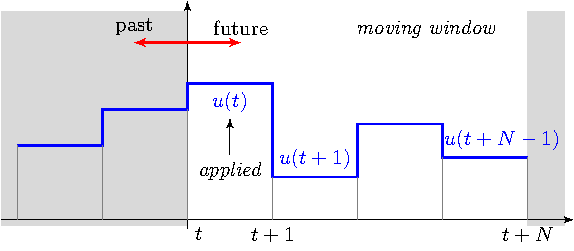
\includegraphics[scale=0.85]{Figures/receding_horizon.pdf}
	\caption{Finite-horizon moving window of MPC: at time $t$, the MPC optimization problem is solved for a finite length window of $N$ steps and the first control input $u(t)$ is applied; the window then recedes one step forward and the process is repeated at time $t+1$.}
	\captionsetup{justification=centering}
	\label{F:MPC-illust}
\end{figure} 
Our main goal is to construct data-driven predictive models for cyber-physical systems that relates the value of the response variable with the values of the predictor variables or features over an horizon with an arbitrary length $N$, and that can also be used to setup a receding horizon control problem. 
In this way we substantially improve the simple mbCRT modeling framework.

Methods based on regression trees are \emph{predominantly} uni-variate output, i.e. defined only for single output variable. 
We introduce a different splitting criteria for trees which enables us to predict multiple outputs. 
If we consider these new outputs as the future states of the single output system, the multi-output tree enables us to implement receding horizon control as the prediction can be made for multiple steps. 
For example, in a building automation case study, one can consider a training dataset with information about the building states like zone temperatures, control set-points and weather conditions, while the output could represented by the power consumption of the building. 
With a single output model, one could estimate the power consumption of the building only at time-step $t$. 
The approach we propose allows to predict the power consumption of the same building at multiple time-steps, i.e. considering a tree with $N+1$ outputs, one could estimate power consumption of the building at $t, t+1,\ldots,t+N$. 
This is termed as look ahead capability of a multi-variate output tree. 
A related case study will be considered in Sec. \ref{sec:case}. 
In this section, we first explain how the regression trees are learned using the CART algorithm, and then modify it into a multi-variate output algorithm to create models that are suitable for finite horizon prediction. 
Finally, we setup a receding horizon control problem based on such models.

\subsection{Predictive modeling with multi-output regression trees}
\label{SS:training_algo}

We use the following notation. We consider a dataset with $n$ observations, where each observation has $s$ features and model has $N$ outputs as
\begin{align}
& x^i := [\x^i_1, \dots, \x^i_s] \in \mathbb{R}^s \nonumber \\
& y^i := [\y^i_1, \dots, \y^i_N] \in \mathbb{R}^N  \label{E:dataset}\\
& i \in \{1,2,\dots, n\}. \nonumber 
\end{align}
Splitting of nodes is shown in Fig. \ref{F:RT}. At $i^{\mathrm{th}}$ node, CART splits the data set into 2 subsets. The left branch $R_L$ contains the data corresponding to $\mathrm{x}_j \leq t_j$ and the right branch $R_R$ corresponding to $\mathrm{x}_j > t_j$. The optimal split at each node is then determined by minimizing the sum of mean square error in both the branches:
\begin{gather}
(\x_k,t_k) = \argmin    \sum_{\{i|\x^i \in R_L\}}{(\y^i_1 - \bar{y}_L)^2}  +  \sum_{\{i|\x^i \in R_R\}} {(\y^i_1 - \bar{y}_R)^2},
\label{E:CART_split_rule}
\end{gather}
where $\bar{y}_L$ and $\bar{y}_R$ are the mean outputs of all the data points in $R_L$ and $R_R$, respectively. The tree is grown in this fashion till the number of data points in the terminal nodes (leaves) exceeds the minimum number of observations in a leaf $minLeaf$, which is often a tuning parameter. Typically a tree is grown till $minLeaf$ size is achieved, and then cost-complexity pruning is employed by collapsing the weak splits \cite{HastieTibshiraniFriedmanEtAl2005}.

\begin{figure}
\centering
\subfigure[First split occurs with input $\x_i$ at $t_i$, second split with input $\x_j$ at $t_j$ and so on, resulting in 5 regions in this case $R_1, \dots, R_5$.]{
\label{F:RT}
\centering
\begin{tikzpicture}[->,>=stealth',level/.style={sibling distance = 3.5cm/#1,
  level distance = 1.5cm}] 
\node [branch_c] {}
    child[blue!50!gray!,thick]{ node [branch_l] {}
            child[blue!50!gray!,thick]{ node [branch_l] {$R_1$} edge from parent node[above left] {$\x_j \leq t_j$}}
            child[red!50!gray!,thick]{ node [branch_r] {$R_2$} edge from parent node[above right] {$\x_j > t_j$}} 
            edge from parent node[above left] {$\x_i \leq t_i$}                            
    }
    child[red!50!gray!,thick]{ node [branch_r] {}
            child[blue!50!gray!,thick]{ node [branch_l] {}
            		child[blue!50!gray!,thick]{ node [branch_l] {$R_4$} edge from parent node[above left] {$\x_k \leq t_k$}}
            		child[red!50!gray!,thick]{ node [branch_r] {$R_5$} edge from parent node[above right] {$\x_k > t_k$}} 
            }
            child[red!50!gray!,thick]{ node [branch_r] {$R_3$}}  
            edge from parent node[above right] {$\x_i > t_i$}    
		}
; 
\end{tikzpicture}
}
\hspace{1cm}
\subfigure[First split occurs with continuous input $\x_i$ at $t_i$, second split with categorical input $\x_j$ at $t_j^r$ such that $\mathcal{S}_{j,L}=\{ t_j^1,\dots,t_j^r \}$ and $\mathcal{S}_{j,R}=\{ t_j^{r+1},\dots,t_j^q \}$.]{
\label{F:RT2}
\centering
\begin{tikzpicture}[->,>=stealth',level/.style={sibling distance = 3.5cm/#1,
  level distance = 1.5cm}] 
\node [branch_c] {}
    child[blue!50!gray!,thick]{ node [branch_l] {}
            child[blue!50!gray!,dashed,thick]{ node [branch_l] {$R_1$} edge from parent node[above left] {$\x_j \in \mathcal{S}_{j,L}$}}
            child[red!50!gray!,dashed,thick]{ node [branch_r] {$R_2$} edge from parent node[above right] {$\x_j \in \mathcal{S}_{j,R}$}} 
            edge from parent node[above left] {$\x_i \leq t_i$}                            
    }
    child[red!50!gray!,thick]{ node [branch_r] {}
            child[blue!50!gray!,thick]{ node [branch_l] {}
            		child[blue!50!gray!,thick]{ node [branch_l] {$R_4$} edge from parent node[above left] {$\x_k \leq t_k$}}
            		child[red!50!gray!,thick]{ node [branch_r] {$R_5$} edge from parent node[above right] {$\x_k > t_k$}} 
            }
            child[red!50!gray!,thick]{ node [branch_r] {$R_3$}}  
            edge from parent node[above right] {$\x_i > t_i$}    
		}
; 
\end{tikzpicture}
}
\caption{Tree structures for (a) only continuous and (b) mix of discrete and continuous variables.}
\captionsetup{justification=centering}
\end{figure}

We extend the same approach to deal with the multi-output data. In order to determine node splits, we are again interested in calculating the splitting variable $\mathrm{x}_k$ and the splitting value $t_k$, but this time we account for errors in all $N$ outputs. Appropriately, we modify \eqref{E:CART_split_rule} as follows:
\begin{gather}
(\mathrm{x}_k,t_k) = \argmin    \sum_{\{i|\x^i \in R_L\}}{||y^i - \bar{y}_L||}_l^2  +  \sum_{\{i|\x^i \in R_R\}} {||y^i - \bar{y}_R||}_l^2,
\label{E:DPC_split_rule}
\end{gather}
where $\bar{y}_L,\bar{y}_R \in \mathbb{R}^N$, and represent the mean $\forall y^i \in R_L$ and $\forall y^i \in R_R$, respectively. 
Norm in this optimization criteria can be chosen to $l^1$ norm if we want to minimize the largest absolute error in the outputs or $l^2$ norm which will minimize the sum of squares across all the outputs. 
We can also introduce weights matrix $Q \in \mathbb{R}^{N \times N}$ as another tuning parameter and choose a quadratic optimization objective:
\begin{gather}
\label{E:DPC_split_rule2}
(\mathrm{x}_k,t_k) = \argmin    \sum_{\{i|\x^i \in R_L\}}{(y^i - \bar{y}_L)}^TQ{(y^i - \bar{y}_L)}  + \sum_{\{i|\x^i \in R_R\}} {(y^i - \bar{y}_R)}^TQ{(y^i - \bar{y}_R)}.
\end{gather}
Both  \eqref{E:DPC_split_rule} and \eqref{E:DPC_split_rule2} can be solved numerically by discretizing the search space of $t_k$ between $max(\mathrm{x}_k)$ and $min(\mathrm{x}_k)$ calculated across $n$ data points. 
The finer the resolution, the better the accuracy of splits. 
The terminating condition for growing the tree remains unchanged in \eqref{E:DPC_split_rule} and \eqref{E:DPC_split_rule2}.

So far, we covered how a tree is built when all the features/variables are continuous. 
It is often the case that some of the features in the data set are categorical, i.e. they can only take discrete values. 
The problem of partitioning a set of discrete values in two subsets is a combinatorial problem. 
Consider a categorical input feature $\mathrm{x}_c$ which can take $q$ different values belonging to the set $\mathcal{S}_c=\{t_c^1,\dots,t_c^q \}$. 
The number of ways to partition $\mathcal{S}_c$ into two non-empty subsets are $2^{q-1}-1$. 
Note that the different possible partitions scale exponentially with $q$, unlike in the continuous case where it grows linearly with resolution. Hence, when $q$ is large, he exact search is not computationally easy to solve. 
We use a near-optimal approach to narrow down this search over all possible partitions. 
The approach is simliar to the one described in \cite{Ripley2007} for single-output system. 
We first find out all $y^i$ corresponding to each element in $\mathcal{S}_c$ and then order the set $\mathcal{S}_c$ according to an increasing mean:
\begin{gather}
\label{E:DPC_cat_split_rule}
\bar{y}_q = \frac{\displaystyle\sum_{\{i|\mathrm{x}_c=t_c^q\}} ||y^i||_l}{N_q},
\end{gather}
where $N_q$ is the number of data points for which $\mathrm{x}_c=t_q$. 
Once $\mathcal{S}_c=\{t_c^1,\dots,t_c^q \}$ is ordered such that 
$\bar{y}_1< \dots < \bar{y}_q$, we split the variable as if it is a continuous variable using \eqref{E:DPC_split_rule} or \eqref{E:DPC_split_rule2} depending upon the chosen type of formulation. 
If the cost is minimized for $\mathrm{x}_c \leq t_c^r$, then the left branch contains $\mathrm{x}_c \in \mathcal{S}_{c,L} = \{ t_c^1,\dots,t_c^r \}$ and the right branch contains $\mathrm{x}_c \in \mathcal{S}_{c,R} = \{ t_c^{r+1},\dots,t_c^q \}$. 
A tree with a mix of continuous and categorical variables is shown in Fig. \ref{F:RT2}. 

In summary, when the dataset contains both types of variables, i.e. continuous and categorical, first the range of all the categorical variables is sorted. 
Then, the optimal cost of splitting is determined for each input feature. 
Finally, the input feature for which this cost is minimum is taken as the splitting variable. Following this approach, we obtain a tree model in the form of
\begin{gather}
[\mathrm{y}_1, \dots, \mathrm{y}_N] = f \left( \mathrm{x}_1, \dots, \mathrm{x}_s \right).
 \label{eq:regtree_multi}
\end{gather}

\subsection{Predictive control with multi-output regression trees}
\label{SS:control_tree}
In this section, we setup a receding horizon control problem using models \eqref{eq:regtree_multi}. 
This algorithm is called Data-driven Predictive Control with Regression Trees (DPCRT). The central idea behind DPCRT is to build tree models which can also predict future states of the system. 
We still use separation of variables as in mbCRT, but train a regression tree with multiple response variables. 
Thus, the difference lies in the number of output variables in each leaf.

Consider $p$ response or output variables $\mathrm{y}_1,\ldots,\mathrm{y}_p$. 
We build $p$ multi-output regression trees. 
Each tree provides the prediction of the corresponding output variable over an horizon of length $N$. 
More precisely, using separation of variables, we first use the methodology proposed in Sec. \ref{SS:training_algo} to train $p$ multi-output regression trees with features $[\mathrm{d}_1,\ldots,\mathrm{d}_{s-m}]\in\mathcal{X}_d$, and then, we fit linear models in the leaves using input variables $u=[\mathrm{u}_1,\ldots,\mathrm{u}_{m}]\in\mathcal{X}_c$, obtaining the following predictive models
\begin{equation}\label{eq:train_model_multi}
y_j := [\mathrm{y}_{j,t}, \ldots, \mathrm{y}_{j,t+N}]^\top = \alpha_{0,i_\mu} + \alpha_{i_\mu} [u(t),\ldots,u(t+N)]^\top,
\end{equation}
where $\alpha_{0,i_j}\in\mathbb{R}^{(N+1)\times 1}$ and $\alpha_{i_j}\in\mathbb{R}^{(N+1)\times m}$ are model coefficients associated with the region/leaf $R_\mu$ of the $j^{th}$ output variable. 
Note that the training procedure can also fit a more complex, e.g. non-linear, model of the input variables instead of \eqref{eq:train_model_multi}, but this worsens the computational complexity. 
We show in Sec.~\ref{sec:case} that the linear models are accurate. 
Once the model is trained, we can setup the following receiding horizon control problem
\begin{equation}\label{eq:DPCRT}
\begin{aligned}
& \underset{u_{t+k} \in \mathcal{X}_c}{\text{minimize}} & &  \sum_{k=0}^{N}{\mathrm{y}^\top_{t+k} \mathrm{Q}\, \mathrm{y}_{t+k} + u^\top_{t+k} \mathrm{R}\, u_{t+k}}  \\
& \text{subject to }                                    & &  \mathrm{y}_{1,t+k}  =  \alpha_{0,i_1} + \alpha_{i_1}[u_t,\ldots,u_{t+k}]^\top                            \\
&                                                       & &  \mathrm{y}_{2,t+k}  =  \alpha_{0,i_2} + \alpha_{i_2}[u_t,\ldots,u_{t+k}]^\top                            \\
&                                                       & &  \vdots                                                                                                   \\
&                                                       & &  \mathrm{y}_{p,t+k}  =  \alpha_{0,i_p} + \alpha_{i_p}[u_t,\ldots,u_{t+k}]^\top                            \\
&                                                       & &  u_{t+k}            \in \mathcal{\bar U}                                                                  \\
&                                                       & &  k                   =   0,\ldots,N.                                                                       \\
\end{aligned}
\end{equation}
We solve this optimization as in the classical MPC formulation, i.e. we apply only the first optimal control input $u(t) = u^*_t$ and proceed to the next time step, where we run the algorithm again with the new measurements.

If the number of control variables is large, the optimization problem \eqref{eq:train_model_multi} may require many data points in the leaves, or in other words a large $minLeaf$, which can affect the accuracy of the regression tree. 
Therefore, we also introduce a variant of this algorithm which will ease the selection of a lower $minLeaf$. 
To do this, we define $h_\nu(y_1,\ldots,y_p),\ \nu=1,2,\ldots$, as some desired functions that relate variables $y_j,\ j=1,\ldots,p$, and setup the following problem
\begin{equation}\label{eq:DPCRTextended}
\begin{aligned}
& \underset{u_{t+k} \in \mathcal{X}_c}{\text{minimize}} & &  \sum_{k=0}^{N}{g(h_1,\ldots,h_m) + u^\top_{t+k} \mathrm{R}\, u_{t+k}}           \\
& \text{subject to }                                    & &  h_1(y_1,\ldots,y_p)  =  \bar \alpha_{0,1} + \bar \alpha_{1}[\mathrm{u}_{1,t},\ldots,\mathrm{u}_{1,t+k}]^\top \\
&                                                       & &  h_2(y_1,\ldots,y_p)  =  \bar \alpha_{0,2} + \bar \alpha_{2}[\mathrm{u}_{2,t},\ldots,\mathrm{u}_{2,t+k}]^\top \\
&                                                       & &  \vdots                                                                                                  \\
&                                                       & &  h_m(y_1,\ldots,y_p)  =  \bar \alpha_{0,m} + \bar \alpha_{m}[\mathrm{u}_{m,t},\ldots,\mathrm{u}_{m,t+k}]^\top \\
&                                                       & &  \mathrm{u}_{j,t+k}   \in \mathcal{\bar U},\ j=1,\ldots,m                                                \\
&                                                       & &  k               =   0,\ldots,N.                                                                          \\
\end{aligned}
\end{equation}
where $\bar \alpha_{0,\nu}\in\mathbb{R}$ and $\bar \alpha_\nu\in\mathbb{R}^{1 \times k}$. 
For example, $h_\nu$ can simply be a linear combination of variables $y_j$ and depends only on the control variable $\u_\nu$. 
With a suitable choice of $g$, both RHC problems \eqref{eq:DPCRT} and \eqref{eq:DPCRTextended} are convex.

Our algorithm for DPC with regression trees in summarized in Algo.~\ref{A:DPC} and a schematic is shown in Fig.~\ref{F:DPC_schematic}.
During the training process, the tree is learned only on disturbance variables with linear models in the leaves, which are a function only of control variables. 
During the control step, at time $t$, the disturbance features $\mathcal{X}_d$ are known for that instant and thus the leaf $R_{\mu}$ is known. 
The optimal control problem is solved to determine the optimal control variables $\left[u^*_t,\dots,u^*_{t+N}\right]$. 
Only the first input $u(t)=u^*_t$ is applied to the system. 
The resulting outputs $\y_{j}(t)$, which form the features for the next time-step, are used to determine the next $R_{\mu}$. 
In the context of a building model, we show the efficacy of DPCRT in Sec. \ref{sec:case}.

\begin{algorithm}[t!]
	\caption{DPCRT: Data-driven Predictive Control with Regression Trees}
	\label{A:DPC}
\begin{algorithmic}[]
			\State \textsc{Design Time}
			\Procedure{Model Training using Separation of Variables}{}
			\State Set $\mathcal{X}_c$ $\gets$ control variables
			\State Set $\mathcal{X}_d$ $\gets$ disturbance variables
			\State Build predictive trees using dataset $(\mathcal{Y},\mathcal{X}_d)$ using \eqref{eq:regtree_multi}
			\ForAll{regions $R_\mu$ at the leaves ofeach tree}
			\State Fit linear model as in \eqref{eq:train_model_multi}
			\EndFor
			\EndProcedure
			\State \textsc{Run Time}
			\Procedure{Predictive Control}{}
			\While{$t< t_{\mathrm{stop}}$}
			\State Determine the leaf and region $R_{\mu}$ using current measurements of $\mathcal{X}_d$
			\State Obtain the linear model at $R_{\mu}$
			\State Solve optimization in \eqref{eq:DPCRT} or \eqref{eq:DPCRTextended} to determine optimal control sequence $[u^*_t,\dots,u^*_{t+N}]^\top$
			\State Apply the first input $u(t)=u^*_t$
			\EndWhile
			\EndProcedure
	\end{algorithmic}
\end{algorithm}
\begin{figure*}[h!]
	\centering
	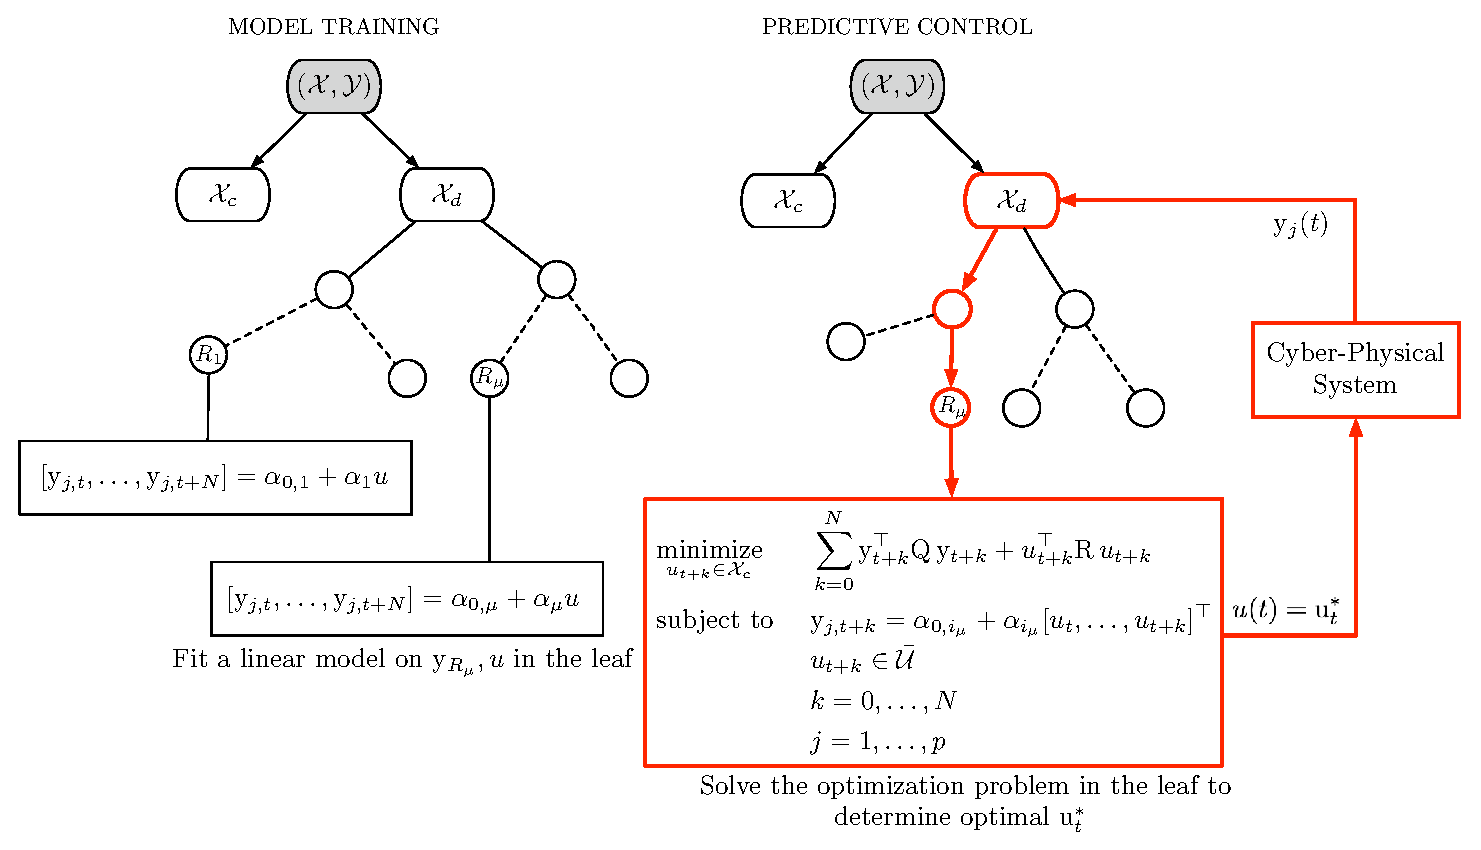
\includegraphics[width=0.9\linewidth]{Figures/DPC_tree.eps}
	\caption{Data Predictive Control with Regression Trees with Model Training Process (left) and Receding Horizon Control (right). During the control step, the optimal control sequence $\left[u^*_t,\dots,u^*_{t+N}\right]^\top $ is determined. The first input $u(t)=u^*_t$ is applied to the system. The resulting output $\y_t$ which is a feature for the next time step is fed back to determine to determine $R_{i}$ at $t+1$.}
	\captionsetup{justification=centering}
	\label{F:DPC_schematic}
\end{figure*}


\section{Case Study: Peak Power Reduction}
\label{sec:case}

In this section, we compare performance of DPCRT against mbCRT with a case study on peak power reduction.
To this aim, we use the DoE Commercial Reference Building (Doe CRB) simulated in EnergyPlus \cite{DeruFieldStuderEtAl2011} as the virtual test-bed building. 
We first describe our test-bed and introduce the data we use, then validate the quality of the DPCRT modeling on the power consumption prediction of DoE CRB, and finally compare DPCRT and mbCRT on the peak power reduction problem.

\subsection{Test-bed description}
DoE CRB is a large $12$ story office building consisting of $19$ zones with a total area of $500,000$ sq.ft. 
There are $2397$ people in the building during peak occupancy. 
During peak load conditions the building can consume up to $1.6$ MW of power. 
For the simulation of the DoE CRB building we use actual meteorological year data from Chicago for the years $2012$ and $2013$. 
The dataset we use for training the trees can be divided into four different categories:
\begin{enumerate}[leftmargin=1cm]
	\item \textbf{Weather Data:} $w = [\mathrm{w}_1,\ldots,\mathrm{w}_d]$. These data include measurements of the outside dry-bulb and wet-bulb air temperature, relative humidity, and wind characteristics. Since we are interested in predicting the power consumption for a finite horizon, we include the weather forecast of the complete horizon in the training features.
	\item \textbf{Schedule Data:} $s = [\mathrm{s}_1,\ldots,\mathrm{s}_r]$. We create proxy variables which correlate with repeated patterns of electricity consumption, e.g. due to occupancy or equipment schedules. For example, Day of Week is a categorical predictor which takes values from $1$ to $7$ depending on the day of the week. This variable can capture any power consumption patterns which occur on specific days of the week. Likewise, Time of Day is quite an important predictor of power consumption as it can adequately capture daily patterns of occupancy, lighting and appliance use without directly measuring any one of them. Besides using proxy schedule predictors, actual building equipment schedules can also be used as training data for building the trees.
	\item \textbf{Building Data:} $b = [\mathrm{b}_1,\ldots,\mathrm{b}_m]$. These data include the states of the building, such as Chilled Water Supply Temperature, Hot Water Supply Temperature, Zone Air Temperature, Supply Air Temperature and Lighting levels.
	\item \textbf{Power Consumption:} $P$. This is the response variable, in addition to zone temperatures. 
\end{enumerate}
In order to predict the power consumption of the building for the entire length of the horizon, we use the notion of auto-regressive trees. An auto-regressive tree is a regular regression tree except that the lagged values of the response variable are also predictor variables for the regression tree, i.e. the tree structure is learned to provide the following model as in \eqref{eq:RTmodel}
\begin{equation}\label{eq:building_model}
P_t = f \left( w(t), s(t), b(t), P(t-1),\dots, P(t-\delta) \right),
\end{equation}
where $\delta$ is the order of the auto-regression and $P(t-j)$ is the value of the power measured at time $t-j$. 
This allows us to make finite horizon predictions of power consumption for the building.

\subsection{DPCRT modeling validation}

Applying \eqref{E:DPC_split_rule2}, we build multi-variate regression trees using a training dataset from July $2012$. 
For a tree with order of auto-regression $\delta = 6$, a prediction horizon $N = 20$ and $\mathrm{Q}$ equal to the identity matrix, the results on the test dataset are shown in Fig. \ref{F:perf_test}. 
The test set shows a day from July 2013. 
In particular, we compare the building power consumption $P_t$ predicted at time $t$, with the actual power consumption of the building from the test dataset. 
Since we can predict the power for multiple steps of the horizon, we add to the comparison the power prediction at time $t$ computed at $t-10$ and $t-20$, i.e. $P_{t|t-10}$ and $P_{t|t-20}$ respectively. 
It can be seen that even with a relatively long horizon, the multi-variate tree model captures the rapid changes in the response variable very accurately. 
DPCRT uses only a subset of features to train the tree, while the inputs are used to train models in the leaves. Thus, the performance of DPCRT depend on two key assumptions
\begin{itemize}[leftmargin=0.5cm]
	\item the separation of variables does not introduce significant errors while training the tree, and
	\item the linear regression at the leaves is a valid assumption.
\end{itemize}
We verify the validity of these assumptions in terms of their effect on model accuracy considering the following two cases:

\begin{figure}
	\subfigure[Building power consumption at time $t$ predicted at time $t$ is denoted by $P(t)$, predicted 10 steps ahead at time $t-10$ is denoted by $P_{t|t-10}$, and predicted 20 steps ahead at time $t-20$ is denoted by $P_{t|t-20}$.]{
		\centering
		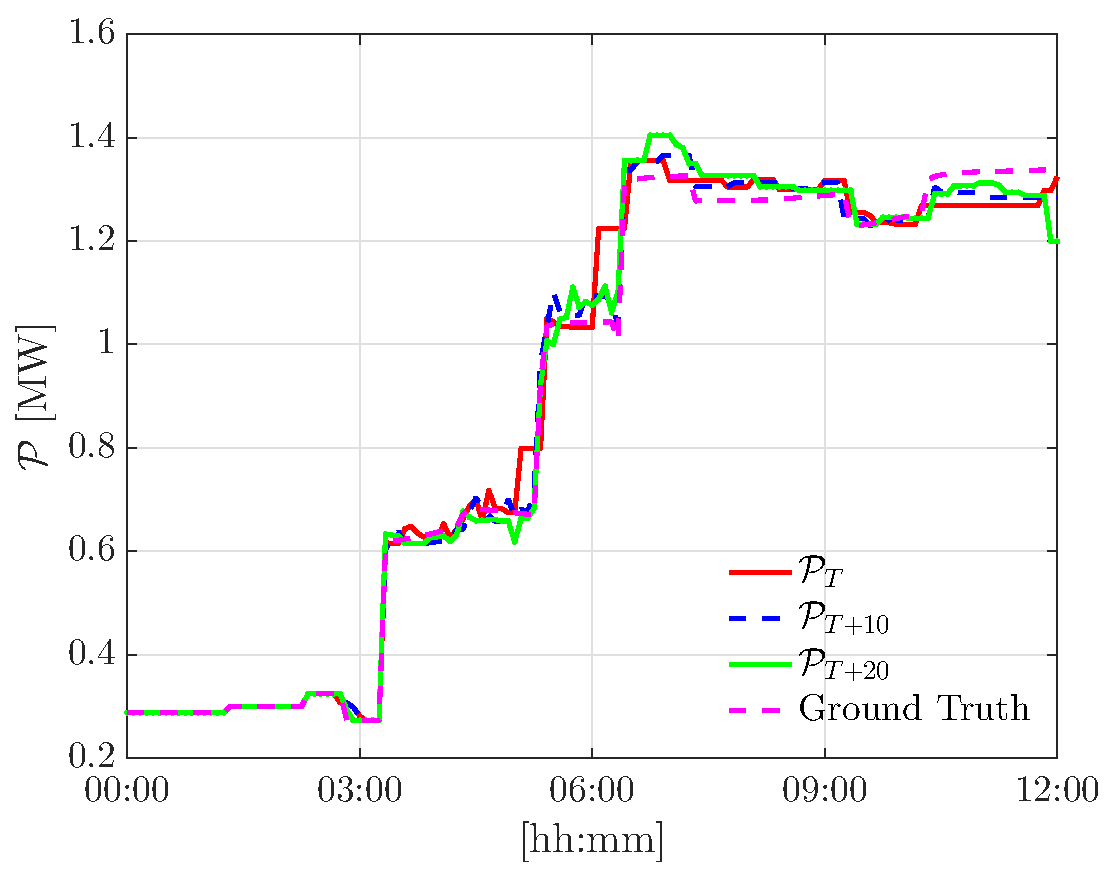
\includegraphics[width=18pc]{Figures/perf_test.eps}
		\label{F:perf_test}
	}
	\subfigure[A comparison of power consumption of the building for two different regression trees. $\mathcal{T}_1$ is trained on all the features while $\mathcal{T}_2$ is trained only on non-manipulated features using separation of variables.]{
		\centering
		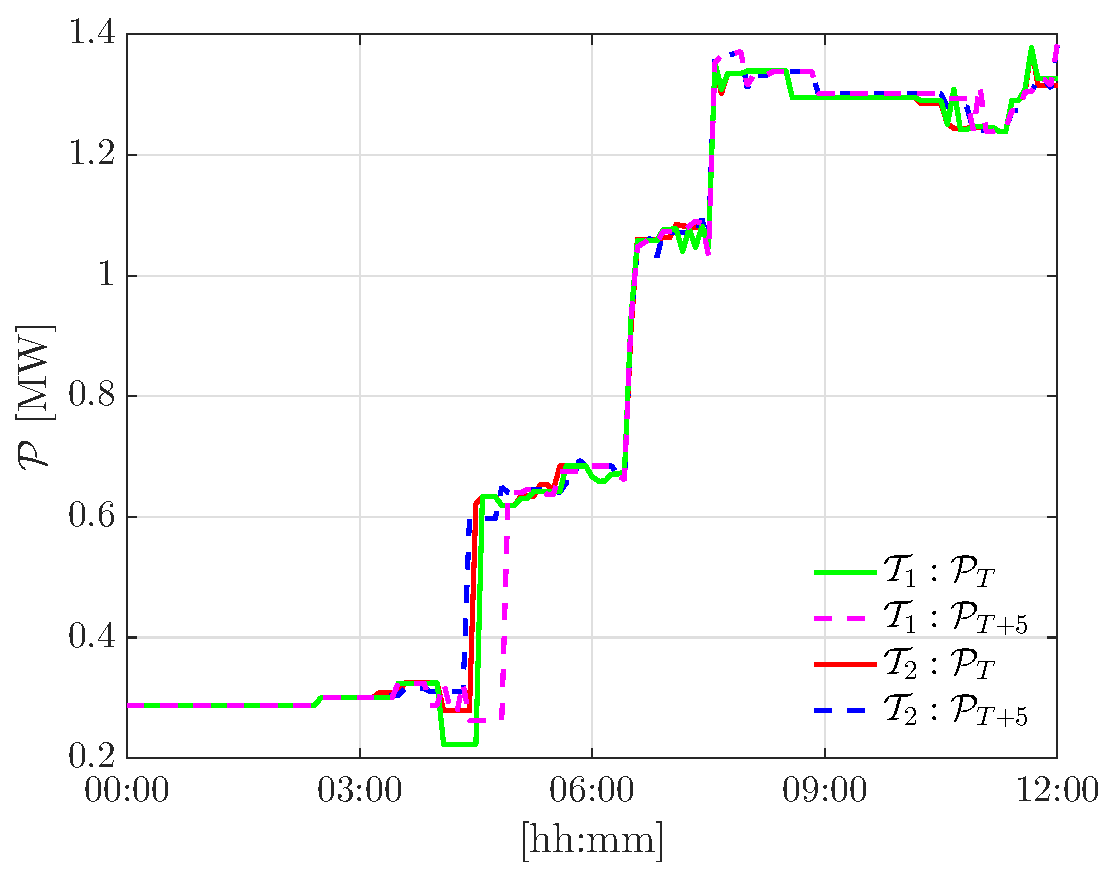
\includegraphics[width=18pc]{Figures/separation_vars.eps}
		\label{F:separation_vars}
	}
	\subfigure[Model validation for linear regression at the leaves of the tree. The predicted and the actual power consumption are very close.]{
		\label{F:linear_approx2}
		\centering
		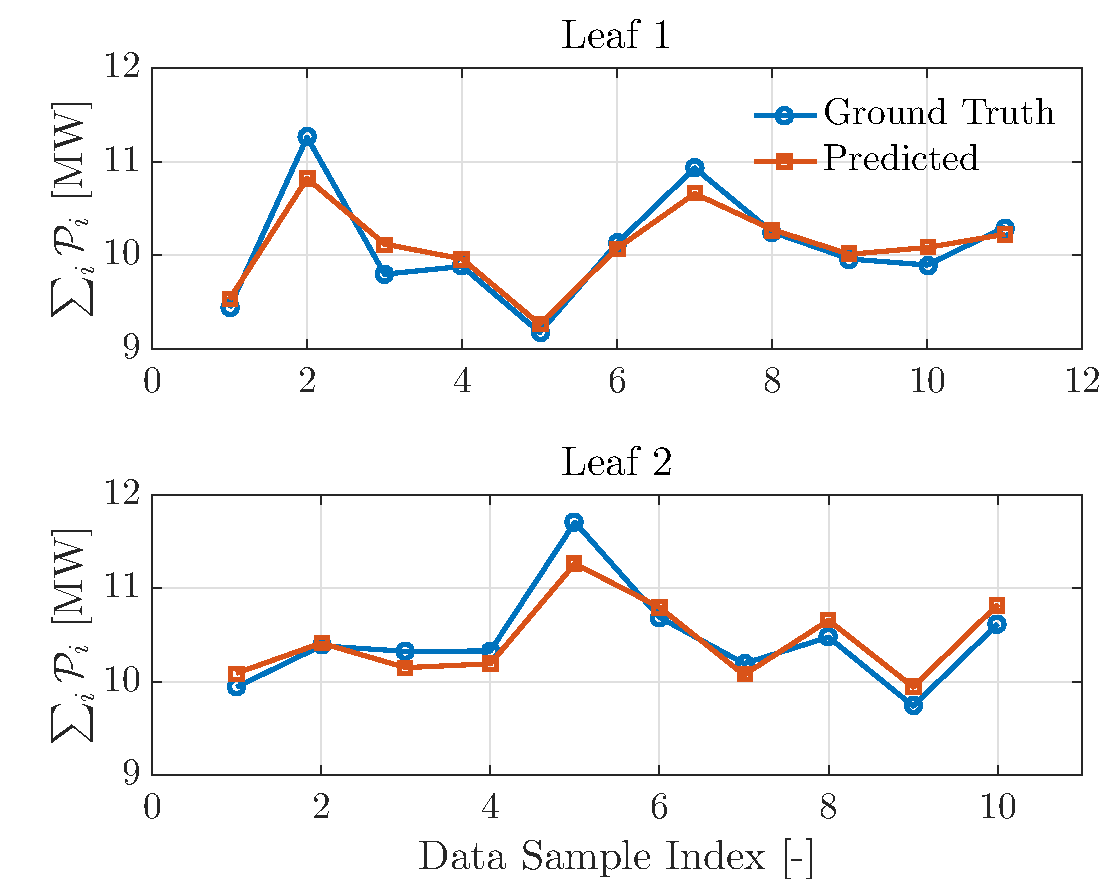
\includegraphics[width=18pc]{Figures/error_leaf2_1.eps}
	}
	\subfigure[The tree has 703 leaves. For each leaf, a maximum and a minimum difference in prediction of average power consumption over the control horizon $P_{\mathrm{pred}}-P_{\mathrm{real}}$ is calculated from the data points that end up in that leaf.]{
		\centering
		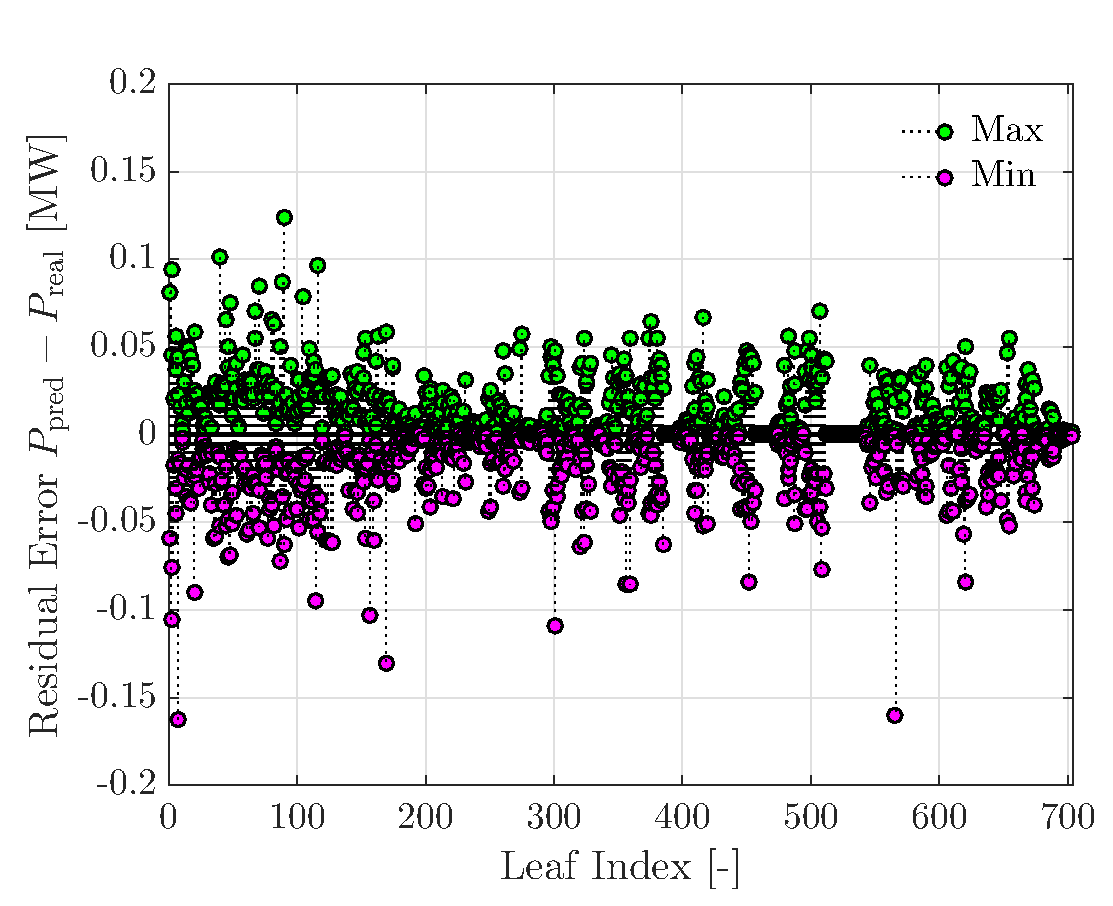
\includegraphics[width=18pc]{Figures/error_leaf.eps}
		\captionsetup{justification=centering}
		\label{F:linear_approx}
	}
	\caption{Model Validation of DPCRT.}
	\captionsetup{justification=centering}
\end{figure}

\begin{enumerate}[leftmargin=1cm]
\item We train $2$ kinds of regression trees: $\mathcal{T}_1$, that is trained using all the features described above, and $\mathcal{T}_2$, that was learned from disturbance variables only, with a linear model on the control variables at the leaves as in \eqref{eq:train_model_multi}.
The predicted power consumption of the building at time $t$ and $t+5$, i.e. $P_t$ and $P_{t+5}$, for both trees is shown in Fig. \ref{F:separation_vars}. 
The normalized root mean square error (NRMSE) for these $2$ outputs on the test dataset is shown in Tab. \ref{T:NMRSE_separation_vars}. 
We notice a small loss in model accuracy with $\mathcal{T}_2$ due to the separation of variables.
This is the cost we have to pay for integrating control synthesis with the tree, since otherwise the control features would have been a part of the splitting criteria rather than a linear model in the leaves of the tree.
\item For the tree $\mathcal{T}_2$, we fit a linear model on the sum of all outputs, i.e. the sum of power consumption over the complete control horizon. For each leaf $i$ we have
\begin{gather}
P_t+ \dots + P_{t+N}  = \beta_{0,i} + \beta_i^\top u.
\end{gather}
For $2$ randomly selected leaves, the fit of the linear model against the actual power consumption is shown in Fig.~\ref{F:linear_approx2}. 
The error observed in the predicted and actual power consumption for all leaves is shown in Fig.~\ref{F:linear_approx}. 
It can be seen that for a small number of samples in the leaves of the tree the linear model assumption is valid.
\end{enumerate}

\begin{table}
	\centering
	\caption{NRMSE for regression trees with and without control features.}
	\begin{tabular}{c|c|c|c|c|c|c}
		\toprule
		& $P_t$ &$P_{t+1}$ &$P_{t+2}$ &$P_{t+3}$ &$P_{t+4}$ & $P_{t+5}$ \\
		\midrule
		$\mathcal{T}_1$     & 0.1037  &  0.1036 &   0.1116 &   0.1124 &   0.1140  &  0.1164  \\
		$\mathcal{T}_2$     & 0.1156  &  0.1182 &   0.1270 &   0.1268 &   0.1324  &  0.1308  \\
		\bottomrule
	\end{tabular}
	\label{T:NMRSE_separation_vars}
\end{table}

\subsection{DPCRT for peak power reduction}

The key to answering the question of what actions to take to achieve a significant DR curtailment upon receiving a notification lies in making accurate predictions about the power consumption response of the building. 
In this context, we evaluate the performance of DPCRT for peak power reduction in buildings, and we show the advantages of receding horizon control with regression trees (DPCRT) with respect to the one-step lookahead control (mbCRT). 

As already described, the data samples consist of four types of features, namely weather data, schedule data, building data and autoregressive terms of building power consumption. 
We use the following three features from the building bata as control variables: zone temperature cooling set point $\mathrm{u}_c$ [$^{\circ}$C], chilled water temperature set point $\mathrm{u}_h$ [$^{\circ}$C], and lighting set point $\mathrm{u}_\ell$ (ranges from $0$ to $1$). Since the power consumption model also depends on the zone temperatures, to have a prediction of the power over the horizon, we first need to predict zone temperatures. To this aim, the following models are built using \eqref{eq:train_model_multi}:
\begin{itemize}[leftmargin=0.5cm]
	\item $P_j^c$ - Power consumption model at time $j$ due to $\mathrm{u}_c$. Learned using all the features except for the inputs. Only $\mathrm{u}_c$ have been used to fit the linear model in the leaves.
	\item $P_j^h$ - Power consumption model at time $j$ due to $\mathrm{u}_h$. Learned using all the features except for the inputs. Only $\mathrm{u}_h$ have been used to fit the linear model in the leaves.
	\item $P_j^\ell$ - Power consumption model at time $j$ due to $\mathrm{u}_\ell$. Learned using all the features except for the inputs. Only $\mathrm{u}_\ell$ have been used to fit the linear model in the leaves.
	\item $T_{i,j}^c$ - Temperature model of the $i^{th}$ room at time $j$ due to $\mathrm{u}_c$. Learned using all the features except for the inputs. Only $\mathrm{u}_c$ have been used to fit the linear model in the leaves.
	\item $T_{i,j}^h$ - Temperature model of the $i^{th}$ room at time $j$ due to $\mathrm{u}_h$. Learned using all the features except for the inputs. Only $\mathrm{u}_h$ have been used to fit the linear model in the leaves.
	\item $T_{i,j}^\ell$ - Temperature model of the $i^{th}$ room at time $j$ due to $\mathrm{u}_\ell$. Learned using all the features. Only $\mathrm{u}_\ell$ have been used to fit the linear model in the leaves.
\end{itemize}

With \(u\) defined as $u=[\u_c,\u_h,\u_\ell]^\top$, we can setup the following DPCRT problem to minimize the peak power consumption
\begin{align}
\begin{aligned}
&\underset{u_{t+k}}{\text{minimize }} && \sum_{k=0}^N \frac{P_{t+k}^c + P_{t+k}^h + P_{t+k}^\ell}{3} +
										  \sum_{k=0}^N \sum_{i=1}^{19} \lambda_i \left(\frac{T_{i,t+k}^c+T_{i,t+k}^h+T_{i,t+k}^{\ell}}{3} - T_{ref} \right)^2      \\ 
&\text{subject to }                   && T_{i,t+k}^c                = \alpha_{0,i}^c + \alpha_{i}^c [\u_{c,t},\ldots,\u_{c,t+k}]^\top, i = 1,\ldots,19             \\
&                                     && T_{i,t+k}^h                = \alpha_{0,i}^h + \alpha_{i}^h [\u_{h,t},\ldots,\u_{h,t+k}]^\top, i = 1,\ldots,19             \\
&                                     && T_{i,t+k}^\ell             = \alpha_{0,i}^\ell + \alpha_{i}^\ell [\u_{\ell,t},\ldots,\u_{\ell,t+k}]^\top, i = 1,\ldots,19 \\
& 									  && \sum_{k=0}^N P_{t+k}^c     = \gamma_0^c + \gamma_1^c [\u_{c,t},\ldots,\u_{c,t+k}]^\top 								   \\
& 									  && \sum_{k=0}^N P_{t+k}^h     = \gamma_0^h + \gamma_1^h [\u_{h,t},\ldots,\u_{h,t+k}]^\top 								   \\
&									  && \sum_{k=0}^N P_{t+k}^\ell  = \gamma_0^\ell + \gamma_1^\ell [\u_{\ell,t},\ldots,\u_{\ell,t+k}]^\top 					   \\
&									  && u_{t+k}                   \in [u_{\mathrm{min}},u_{\mathrm{max}}] 																		   \\ 
&									  &&  k                         =  0, \ldots, N.                                                                                \\
\end{aligned}
\label{eq:DPCRTCaseStudy}
\end{align}
At time $t$, we solve DPCRT \eqref{eq:DPCRTCaseStudy} and apply only the first input, i.e. $\u_c(t) = \u^*_{c,t}$, $\u_h(t) = \u^*_{h,t}$ and $\u_\ell(t) = \u^*_{\ell,t}$. At $t+1$, we repeat the algorithm with the updated measurements.

We compare DPCRT and mbCRT when simulated in closed-loop with the EnergyPlus model of the building. In order to compare the performance of DPCRT, we consider a scenario in which there is a significant disturbance which is only anticipated $30$ min in advance and leads to a sudden increase in zone temperatures in the building. This maybe due to a sudden spike in the occupancy or equipment being switched ON at a brief notice. Under this scenario, it is important to react to the disturbance in a predictive manner in order to minimize the peak power consumption. This scenario is shown in Fig. \ref{F:scenario}. Between $15:30$ and $16:00$, an enormous spike in the power consumption ($1.5\times$) is expected because of a scheduled operation.
\begin{figure*}
	\centering
	\hspace{1pt}
	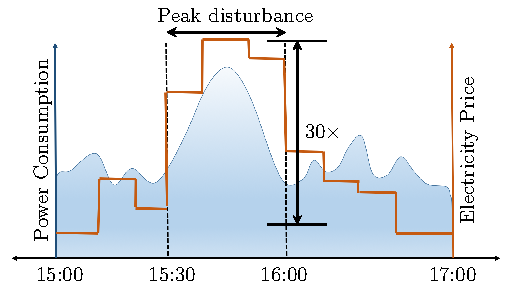
\includegraphics[width=0.5\textwidth]{figs/peakpowerplot.pdf}
	\centering
	\caption{Peak disturbance between $1530-1600$ hours. The test scenario used in the DPCRT case study simulations has a $1.5\times$ peak disturbance between $15{:}30$ and $16{:}00$.}
	\label{F:scenario}
	\vspace{-10pt}
\end{figure*}
\begin{figure}[b!]
\centering
\subfigure[Control strategies.]{
\centering
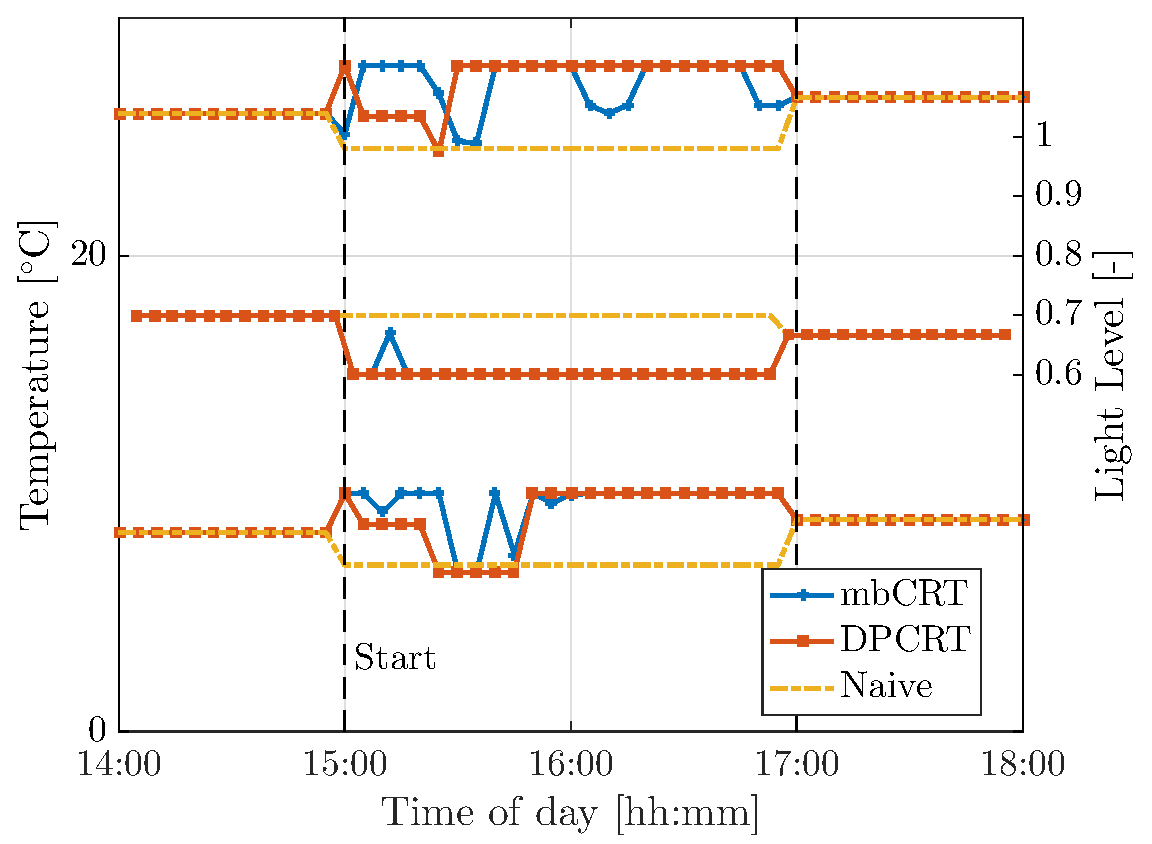
\includegraphics[width=18.5pc]{Figures/res_control.eps}
\label{F:res_control}
}
\subfigure[Power consumption.]{
\centering
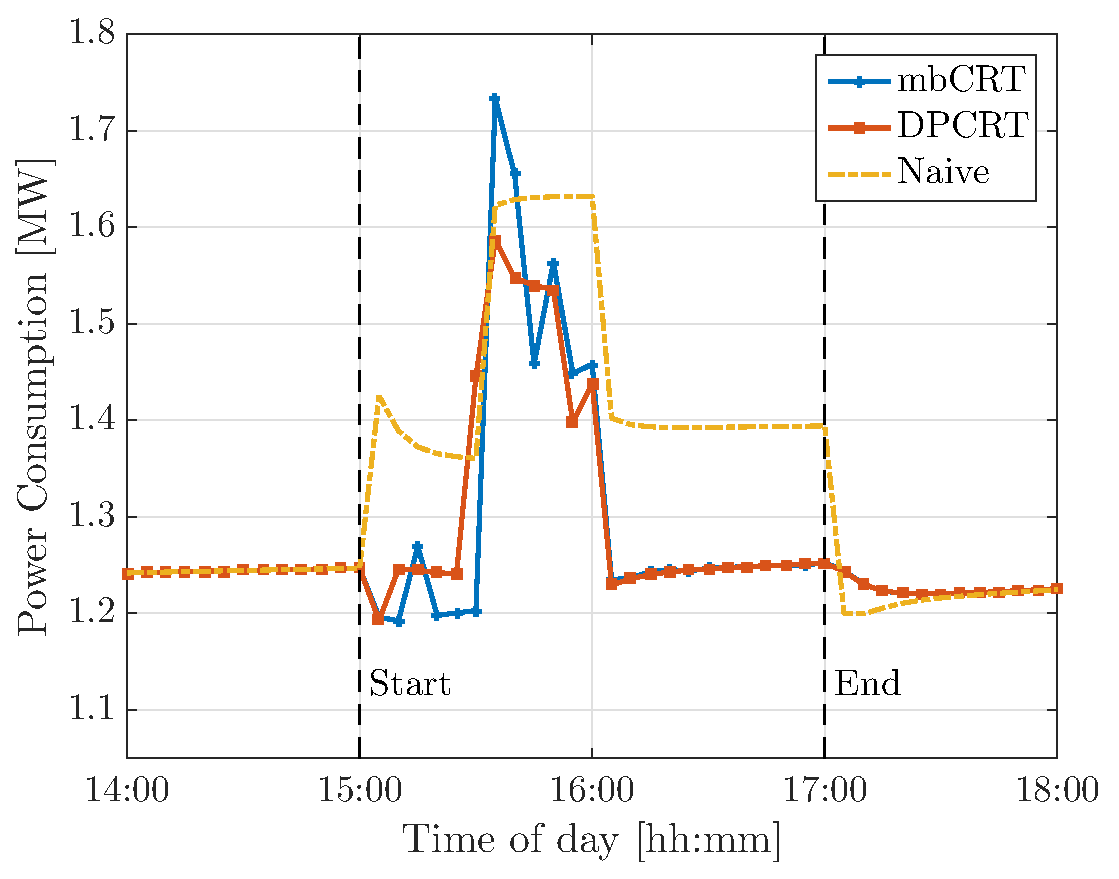
\includegraphics[width=18.5pc]{Figures/res_power.eps}
\label{F:res_power}
}
\caption{A comparison between mbCRT and DPCRT along with a Naive rule-based strategy.}
\captionsetup{justification=centering}
\end{figure}
The control strategies are tested over a $2$ hours duration between $15{:}00$ and $17{:}00$. Fig. \ref{F:res_control} shows $3$ control strategies: mbCRT, DPCRT and a Naive load reduction strategy. The naive strategy is equivalent to not responding to the disturbance at all. It maintains the desired zone temperature set point $\u_c$, chiller water temperature set point $\u_h$ and lighting level $\u_\ell$ throughout the test period. In Fig. \ref{F:res_power}, it can be seen that DPCRT reacts to the disturbance much before mbCRT, which waits until the last time-step before the disturbance to react. This leads to a significantly lower peak power consumption that mbCRT. In the case of DPCRT, the control horizon is $6$. At $15{:}00$, DPCRT strategy is same as the greedy one. At $15{:}05$, the downstream disturbance is visible to DPCRT algorithm and it starts to pre-cool the building by decreasing both cooling and chiller water set points. At $15{:}25$, the $\u_c$ and the $\u_h$ are reduced to minimum so that in the period of extreme disturbance an optimal trade-off between power consumption and thermal comfort is maintained. Thus, DPCRT algorithm foresees the disturbance and takes a preemptive action against it.  On the other hand, the mbCRT algorithm considers the power consumption and the zone temperatures of only one time step. Therefore, it does not know of an upcoming disturbance. At every time step, it chooses that $\u_c$, $\u_h$ and $\u_\ell$ which optimizes the cost for that time step. Naturally, this leads to a jaggy behavior in the control strategy. We can see a similar behavior for the power consumption in Fig. \ref{F:res_power}. The DPCRT algorithm gradually increases the power consumption because it can see the disturbance before it actually reaches $15{:}30$, while in the case of mbCRT, the power consumption overshoots by a big margin because the controller deals with the disturbance in a single step. DPCRT maintains zone temperature much closer to the reference temperature of $24^oC$ while both mbCRT and the naive strategy have large deviations from the desired temperature. 

The quantitative comparison is presented in Tab. \ref{T:case_quant}. Between $15{:}00$ and $17{:}00$, DPCRT and mbCRT result in similar energy usage, $5102$ kWh and $5097$ kWh, respectively, both outperforming the Naive strategy which incurs $5358$ kWh. Peak power in the case of DPCRT is $1.58$ MW which is lower than both mbCRT ($1.73$ MW) and the Naive strategy ($1.63$ MW), although Naive outperforms mbCRT. The peak power with DPCRT is $8.6\%$ less than mbCRT and $3.1\%$ less than the Naive. While both DPCRT and mbCRT account for thermal comfort, DPCRT deviates less from the desired temperature. The Naive strategy does not trade-off on the thermal comfort. Thus, DPCRT outperforms mbCRT both in terms of a reduced peak power consumption and better thermal comfort.

\begin{table}
  \centering
  \caption{Quantitative comparison for Energy Consumption, Peak Power and $\%$ Reduction in Peak Power of DPCRT compared to Naive approach and mbCRT.}
    \begin{tabular}{c|c|c|c}
    \toprule
     & Energy & Peak Power & Peak                       \\
     & [kWh]  & [MW]       & Reduction                  \\     
    \midrule
    Naive     & $5358$     &  $1.63$ &   $3.1\%$        \\
    mbCRT     & $5097$     &  $1.73$ &   $\bold{8.6\%}$ \\
    DPCRT     & $5102$     &  $1.58$ &   -              \\
    \bottomrule
    \end{tabular}
  \label{T:case_quant}
\end{table}


\section{Conclusion}
\label{sec:discussion}
We present a data-driven approach for control-oriented modeling of large-scale cyber-physical systems. 
%We show how regression trees are well suited to address challenges associated with Demand-Response for large \textit{C/I/I} consumers while being interpretable. 
We present a data-driven predictive control with regression trees (DPCRT) -- an algorithm for implementing receding horizon control. 
DPCRT enables optimal control designs for complex problems which otherwise are dependent on expensive first principles or physics-based models. 
We apply DPCRT to the problem of peak power reduction in buildings in context of Demand Response. 
The performance of DPCRT are evaluated on a DoE commercial reference virtual test-bed. 
%It results in a much lower energy consumption when compared to the Naive control strategy. 
Results show that it provides a smooth and much lower power consumption while maintaining a desired thermal comfort level for every zone.
In the considered example, DPCRT leads to $8.6\%$ decrease in the peak power consumption of the building when compared to the mbCRT algorithm (one-step look ahead) and $3.1\%$ decrease when compared to a Naive rule-based reduction strategy. 
These advantages make DPCRT an alluring tool for evaluating and planning DR curtailment responses for large scale cyber-physical energy systems.
The approach we propose in this paper modifies the CART algorithm considering the error minimization of the system evolution over a predictive horizon. 
This results in a multi-output regression tree modeling that is extremely simple from the computational complexity point of view. 
To improve the accuracy of our algorithms, new methods based on Random Forests are currently under investigation. Preliminary results can be found in \cite{JainACC2017,JainCDC2017}.



%\let\secfnt\undefined
%\newfont{\secfnt}{ptmb8t at 10pt}

\bibliographystyle{unsrt}
\bibliography{references,ref_buildsys,newrefs}

\end{document}


